\section{Obiettivo}

L'obiettivo di questa relazione \`{e} quello di realizzare un'implementazione di un \textbf{ambiente} di \textbf{Reinforcement Learning} per allenare un agente, tramite un algoritmo di \textbf{Q-Learning}, a muoversi in modo "\textit{intelligente}" all'interno di un labirinto, ovvero l'agente deve essere in grado di non andare a sbattere contro le mura del labirinto e possibilmente arrivare all'uscita.

\section{Ipotesi iniziali e vincoli}
L'agente si trover\`{a} all'interno di un ambiente bidimensionale (griglia 2D) formato da svariate celle che possono essere di due tipi:

\begin{enumerate}
	\item \textbf{Celle Vuote}: in questo tipo di celle l'agente pu\`{o} muoversi liberamente e rappresentano uno spazio vuoto/percorribile del labirinto
	\item \textbf{Celle Muro}: queste celle rappresentano un muro del labirinto e l'agetne non pu\`{o} attraversarle o fermarcisi sopra, l'unica cosa che pu\`{o} fare \`{e} evitarle.
\end{enumerate}
\ \\
L'insieme di tutte le \textit{Celle Vuote} e \textit{Celle Muro} forma il \textbf{labirinto} che pu\`{o} essere visto come una matrice di dimensione $m \times n$, dove $m$ \`{e} il numero di righe ed $n$ il numero di colonne.

\begin{equation*}
\large
Maze_{m \times n}=
\begin{bmatrix}
a_{0,0} & \cdots & a_{0,n-1} \\
\vdots & \cdots & \vdots \\
a_{m-1,0} & \cdots & a_{m-1,n-1}
\end{bmatrix}
\end{equation*}
\captionof{figure}{Esempio di labirinto di dimensione $m \times n$}
\ \\
L'agente inizier\`{a} sempre dalla prima cella in alto a sinistra $a_{0,0}$ (\textit{start position}) e dovr\`{a} raggiungere l'ultima cella in fondo a destra $a_{m-1,n-1}$ (\textit{goal position})  muovendosi solo tra le celle a lui vicine (quelle visibili dal vicinato di \textit{Von Neuman}) e mai in diagonale ! Non sar\`{a} neanche in grado di spostarsi in celle al di fuori di quelle della matrice e.g. $a_{-1, 0}$ e non si verificher\`{a} \textit{l'effetto pacman}, cio\`{e} l'agente non potr\`{a} effettuare mosse del tipo: $ a_{1,n-1} \ \rightarrow \ a_{1, 0}$

\begin{equation*}
\large
\begin{matrix}
	\ & a_{4,4} & \ \\
	a_{5,3} & a_{5,4} & a_{5,5}\\
	\ & a_{6,4} & \ \\
\end{matrix}
\end{equation*}
\captionof{figure}{Esempio di vicinato di Von Neuman dove l'agente si trova in posizione $5, 4$}
\ \\
L'ambiente, ad ogni mossa dell'agente, ritorner\`{a}  \textit{un'osservazione} formata dalle celle a lui vicine (questa volta con il vicinato di Moore) nella sua nuova posizione e un \textit{reward} in base alla bont\`{a} dell'azione effettuata:

\begin{itemize}
	\item $-1$: una qualunque mossa in una cella vuota
	\item $-5$: una mossa contro un muro (equivale a rimanere fermo sul posto)
	\item $+10$: raggiungere la cella goal
\end{itemize}

\begin{equation*}
	\large
	\begin{matrix}
		a_{ 4,3} & a_{4,4} & a_{4,5} \\
		a_{5,3} & a_{5,4} & a_{5,5}\\
		a_{6,3} & a_{6,4} & a_{6,5} \\
	\end{matrix}
\end{equation*}
\captionof{figure}{Esempio di vicinato di Moore dove l'agente si trova in posizione $5, 4$}

\subsection{Vincoli dell'agente}
In breve tutti i vincoli dell'agente:

\begin{itemize}
	\item Pu\`{o} muoversi solo nelle \textbf{Celle Vuote}
	\item Non pu\`{o} oltrepassare le \textbf{Celle Muro} e muoversi contro una di queste equivale a rimanere fermo sul posto
	\item Non pu\`{o} uscire dalle mura del labirinto (non pu\`{o} andare fuori dalle celle della matrice e.g. $a_{-1, 0}$)
	\item Non esiste \textit{l'effetto pacman}
	\item Le azioni che pu\`{o} compiere sono: \lstinline[style=cmd]|UP, DOWN, LEFT, RIGHT|
	\item Pu\`{o} muoversi solo nelle celle a lui vicine e non in diagonale (vicinato di Von Neuman)
\end{itemize}

\subsection{Vincoli dell'ambiente}
\label{sec:vincoliambiente}
In breve i vincoli dell'ambiente:

\begin{itemize}
	\item L'ambiente \`{e} rappresentato tramite una griglia 2D (matrice)
	\item L'ambiente ha dimensione $m \times n$ dove $m$ \`{e} il numero di righe ed $n$ il numero di colonne.
	\item La \textit{starting position} \`{e} sempre la prima cella in altro a sinistra: $a_{0,0}$
	\item La \textit{goal position} \`{e} sempre l'ultima cella in fondo a destra: $a_{m-1, n-1}$
	\item Ritorna all'agente un'\textit{osservazione} data dal vicinato di Moore della posizione dell'agente
	\item Ritorna un \textit{reward} all'agente in base alla bont\`{a} della mossa: 
		\begin{itemize}
			\item[*] $-1$: una qualunque mossa in una cella vuota
			\item[*] $-5$: una mossa contro un muro (equivale a rimanere fermo sul posto)
			\item[*] $+10$: raggiungere la cella goal
		\end{itemize}
\end{itemize}

\section{Struttura e file del progetto}
\label{sec:progetto}

\textbf{Nota:} Tutto il codice mostrato successivamente \`{e} disponibile nella seguente repo github: \href{https://github.com/ncvescera/QRL-Maze_in_a_Wall}{QRL-Maze\_in\_a\_Wall}.\\

La seguente \`{e} una breve anteprima di come si presenta la cartella del progetto:

\begin{center}
	\begin{tabular}{m{15em}  m{20em}}
		
\includegraphics[height=0.8em]{img/paper.png} \lstinline[style=cmd]|main.py| & \textit{Script principale}\\[0.2em]
		\hline 
		
\includegraphics[height=0.8em]{img/paper.png} \lstinline[style=cmd]|MazeEnv.py| & \textit{Rappresentazione dell'ambiente} \rule{0pt}{2.6ex}\\
		\hline
		
\includegraphics[height=0.8em]{img/paper.png} \lstinline[style=cmd]|QLearning.py| & \textit{Algoritmo di QLearning} \rule{0pt}{2.6ex}\\
		\hline
		
\includegraphics[height=0.8em]{img/paper.png} \lstinline[style=cmd]|GUI.py| & \textit{Responsabile della GUI} \rule{0pt}{2.6ex}\\
		\hline
		
\includegraphics[height=0.8em]{img/paper.png} \lstinline[style=cmd]|generate_dataset.py| & \textit{Crea il dataset} \rule{0pt}{2.6ex}\\
		\hline
		
\includegraphics[height=0.8em]{img/paper.png} \lstinline[style=cmd]|training.py| & \textit{Script per allenare l'agente} \rule{0pt}{2.6ex}\\
		\hline
		
\includegraphics[height=0.8em]{img/paper.png} \lstinline[style=cmd]|testing.py| & \textit{Script per valutare l'agente} \rule{0pt}{2.6ex}\\
		\hline
		
\includegraphics[height=0.8em]{img/paper.png} \lstinline[style=cmd]|maze_utils.py| & \textit{Funzioni utilities} \rule{0pt}{2.6ex}\\
		\hline
		
\includegraphics[height=0.8em]{img/paper.png} \lstinline[style=cmd]|maze.txt| & \textit{File per rappresentare una labirinto} \rule{0pt}{2.6ex}\\
		\hline
		
\includegraphics[height=0.8em]{img/paper.png} \lstinline[style=cmd]|Qmatrix| & \textit{Matrice per QLearning} \rule{0pt}{2.6ex}\\
	\end{tabular}
\end{center}

\begin{itemize}
	\item Il file \lstinline[style=cmd]|MazeEnv.py|, che conterr\`{a} l'omonima classe, \`{e} il responsabile della modellazione dell'ambiente. Questo si occuper\`{a}  di verificare le mosse dell'agente, di assegnare i reward e di ritornare a quest'ultimo le osservazioni dell'ambiente che lo circonda.
	\item \lstinline[style=cmd]|QLearning.py| ha il compito di gestire la \textit{matrice Q }: salvarla su apposito file e caricarla in memoria, gestire la fase di allenamento (\textit{training}) e di esecuzione (\textit{testing/execution}). \`{E} qui che risiede l'algoritmo di QLearning vero e proprio.
	\item \lstinline[style=cmd]|GUI.py|, questa classe ha il compito di stampare a video il labirinto e le varie mosse dell'agente. Pu\`{o} farlo in due modi: 
	\begin{enumerate}
		\item \textbf{GUI}: tramite una finestra dove il labirinto viene rappresentato a colori
		\item  \textbf{CLI}: direttamente nel terminale con soli caratteri testuali
	\end{enumerate}
	\item \lstinline[style=cmd]|generate_dataset.py| \`{e} responsabile della creazione del dataset: 100 labirinti generati in modo casuale con dimensione massima $10 \times 10$, minima di $3 \times 3$ ed un numero casuale di mura, per il \textit{training} e 20, costruite allo stesso modo delle precedenti, per il \textit{testing/execution}.
	\item \lstinline[style=cmd]|training.py| avvia la fase di \textit{training} e permette all'utente di scegliere alcuni parametri come:
	\begin{itemize}
		\item Numero di Epoche
		\item Numero di Step
		\item Se utilizzare il dataset di training o una matrice definita dall'utente
		\item Se continuare l'allenamento (e quindi caricare la \textit{matrice Q} gi\`{a} esistente andando a modificarla) o iniziarne uno nuovo daccapo (creare una nuova \textit{matrice Q} e popolarla)
	\end{itemize}
	In questa fase non \`{e} prevista la stampa \textit{GUI} e se utilizzato il dataset di training, per ogni matrice verr\`{a} salvato un grafico che mostra il risultato dell'allenamento.
	\item \lstinline[style=cmd]|testing.py| permette all'utente di eseguire la fase di \textit{testing/execution} dandogli la possibilit\`{a} di scegliere:
	\begin{itemize}
		\item se utilizzare la modalit\`{a} \lstinline[style=cmd]|step-by-step| (possibilit\`{a} di eseguire un'azione alla volta e anche di scegliere quale azione fare per ogni stato) o l'esecuzione automatica
		\item se utilizzare la stampa \textit{GUI} o \textit{CLI}
		\item se avviare l'esecuzione con una matrice generata dall'utente o con il dataset di testing
	\end{itemize}
	\item \lstinline[style=cmd]|maze_utils.py| insieme di funzioni utili per la gestione del labirinto, come la generazione casuale di quest'ultimi, la possibilit\`{a} di salvare un labirinto su file o di caricarlo in memoria.
	\item \lstinline[style=cmd]|main.py| punto iniziale per avviare l'intero progetto, permette all'utente di scegliere quale parte del progetto avviare e testare.
	\item \lstinline[style=cmd]|maze.txt| file che contiene una matrice definita dall'utente. Tutte le celle delle matrici sono popolate da \lstinline[style=cmd]|0| o \lstinline[style=cmd]|1|, che rispettivamente indicano una \textbf{Cella Vuota} e una \textbf{Cella Muro}.
	\item \lstinline[style=cmd]|Qmatrix| la matrice creata durante la fase di addestramento.
\end{itemize}

\subsection{maze.txt}

Prima di iniziare ad analizzare il codice in se, \`{e} necessario dare uno sguardo a come i labirinti vengono rappresentati. Sia il file \lstinline[style=cmd]|maze.txt| (che viene creato e popolato dall'utente), sia i file generati dallo script per la creazione del dataset, hanno lo stesso formato: un insieme di \lstinline[style=cmd]|0| e \lstinline[style=cmd]|1| separati da spazi disposti su pi\`{u} righe. Questi numeri indicano rispettivamente: una \textbf{Cella Vuota} e una \textbf{Cella Muro}.
Di seguito alcuni esempi di labirinti validi e non:\\

\begin{tabular}{m{20em}  m{20em}}
\begin{lstlisting}[style=python, caption={Labirinto 8x9 valido}, label={lst:valido1}]
	0 0 0 0 0 0 0 0 0
	0 1 1 1 1 1 1 1 1
	0 0 1 0 0 0 0 0 0
	0 0 1 0 1 0 0 0 0
	0 0 1 0 1 0 0 0 0
	0 0 0 0 1 0 0 0 0
	0 0 0 0 1 0 0 0 0
	0 0 0 0 1 0 0 0 0
\end{lstlisting}
&
\begin{lstlisting}[style=python, caption={Labirinto 5x7 valido}, label={lst:valido2}]
	0 0 0 0 0 0 0
	0 1 0 1 0 0 0
	0 0 0 1 0 0 1
	0 0 1 0 1 0 0
	0 0 0 0 0 0 0
	
	
	
\end{lstlisting}
\end{tabular}

\begin{tabular}{m{20em}  m{20em}}
	\begin{lstlisting}[style=python, caption={Labirinto 4x4 NON valido}, label={lst:novalido1}]
		0 1 0 0
		1 1 0 0
		0 0 0 0
		0 1 0 0
	\end{lstlisting}
	&
	\begin{lstlisting}[style=python, caption={Labirinto 4x5 NON valido}, label={lst:novalido2}]
		0 0 0 0 0
		1 1 0 0 0
		0 0 0 1 1
		0 1 0 1 0
	\end{lstlisting}
\end{tabular}

I labirinti \ref{lst:valido1} e \ref{lst:valido2} risultano validi in quanto l'agente (che parte dalla prima cella in alto a sinistra) riesce sempre a raggiungere lo stato goal (ultima cella in basso a destra), mentre nel labirinto \ref{lst:novalido1} l'agente risulta bloccato alla partenza ed in nessuno modo riuscir\`{a} ad uscire dalla sua "prigione". Stessa cosa vale per il \ref{lst:novalido2} dato che non riuscir\`{a} mai a raggiungere il goal.

\subsection{maze\_utils.py}
All'interno di questo file sono presenti alcune funzioni "\textit{utilities}" per la generazione, controllo e caricamento dei labirinti. 

\subsubsection{is\_solvable}
\`{E} proprio qui che le varie matrici vengono controllate e ottengono lo stato di \textit{valide/risolvibili} (\textit{solvable}). 
Questo controllo viene fatto tramite un'esplorazione in ampiezza (\textit{BFS}) che percorre tutto il labirinto e ritorna \lstinline[style=cmd]|True| se l'agente riesce ad arrivare allo stato goal, altrimenti \lstinline[style=cmd]|False|. Questo controllo non intacca di molto le performance dell'algoritmo in quanto anche su matrici $10 \times 10$ il suo tempo di completamento non \`{e} minimamente rilevante: 

\begin{figure}[H]
	\centering
   	\begin{tabular}{c | c | c | c | c | c}
		 & $3 \times 3$ & $6 \times 6$ & $10 \times 10$ & $50 \times 50$ & $100 \times 100$\\
		\hline
		\textbf{Tempo} (s) & 0.0 & 0.0 & 0.0 & 0.0 & 0.0\\ [2em]
	\end{tabular}
	\caption{Tempi di esecuzione della funzione \lstinline[style=cmd]|is_solvable()| con matrici di diversa dimensione.}
\end{figure}

Il costo in tempo \`{e} $O(mn)$:

\begin{center}
	$Tcosto = O(V + E) = O(mn + mn - n + mn - m) = O(3mn - m - n) = O(mn) $
\end{center}
$dove: $
\begin{itemize}
	\item $V = mn$
	\item $E = (n)(m-1) + (m)(n-1)$
\end{itemize}

Anche il costo in spazio \`{e} identico in quanto la lista \lstinline[style=cmd]|seen| sar\`{a} grande al pi\`{u} $m \times n$.

\begin{lstlisting}[style=python, caption={Funzione per controllare la risolvibilit\`{a} dei labirinti}]
	def is_solvable(maze) -> bool:
		x, y = maze.shape
		
		start_position = (0, 0)
		end_position = (x-1, y-1)

		seen = {start_position}     # elementi visitati
		queue = [start_position]    # coda di elementi da visitare
	
		while queue:
			i, j = queue.pop(0)
			seen.add((i, j))
	
			for di, dj in [(1, 0), (-1, 0), (0, 1), (0, -1)]:
				ni, nj = i+di, j+dj   # nuova posizione del vicino
				
				if (ni, nj) in seen:
					continue	# se e' gia' stato visitato
	
				elif ni < 0 or nj < 0 or ni >= len(maze) or nj >= len(maze[0]):
					continue	# se e' fuori dalla matrice
	
				elif ni == end_position[0] and nj == end_position[1]:
					return True		# se e' arrivato alla fine
	
				elif maze[ni][nj] == 1:
					continue	# se e' un muro
	
				else: 	# se e' una casella libera
					seen.add((ni, nj))      # aggiunge alla lista visitati
					queue.append((ni, nj))  # aggiunge alla coda da visitare
	
		return False
\end{lstlisting}
\pagebreak
\subsubsection{grid\_from\_file}
La funzione che si occupa di caricare in memoria un labirinto da file risulta essere abbastanza banale: tenta di aprire il file \lstinline[style=cmd]|maze.txt|, se non esiste o il suo contenuto \`{e} errato o il labirinto al suo interno non \`{e} risolvibile ritorna \lstinline[style=cmd]|None| ed un messaggio di errore, altrimenti ritorna la matrice sotto forma di \lstinline[style=cmd]|numpy.ndarray|.

\begin{lstlisting}[style=python, caption={Funzione per il caricamento in memoria di un labirinto da file}]
	def grid_from_file(filename: str) -> tuple[np.ndarray, str]:
		grid = None
		message = ""
	
		try:
			grid = np.loadtxt(filename, dtype=int)
		except FileNotFoundError:
			grid = None
			message = "File inesistente !"
			return grid, message
	
		# il file esiste ma risulta vuoto
		if grid is not None and grid.size == 0:
			grid = None
			message = "Il contenuto del file e' errato !"
	
		elif not is_solvable(grid):
			grid = None
			message = "Il labirinto non e' risolvibile !"
	
		return grid, message
\end{lstlisting}

\subsubsection{generate\_grid}
La funzione \lstinline[style=cmd]|generate_grid| riesce a creare labirinti, di dimensione e numero di mura date, sempre risolvibili. Ci riesce in quanto controlla sempre se sta generando un muro in una posizione che non dovrebbe (cella \textit{start} e \textit{goal}) (nel caso non crea il muro e lo rigenera casualmente) ed il numero massimo di mura inseribili \`{e} pari a: 

\[maxWalls = \frac{m * n}{2}\]

Superando $maxWalls$ si potranno andare a generare barriere  di mura insuperabili dall'agente, ma restando sotto questo limite \`{e} sempre certo che questo fenomeno non accadr\`{a} mai.
\pagebreak
\begin{lstlisting}[style=python, caption={Funzione per la generazione di labirinti casuali}]
	def generate_grid(m, n, walls=10) -> np.ndarray:
		if walls >= (m * n / 2):
			print("Non e' possibile generare un labirinto esplorabile !!!")
			return None
	
		solvable = False
		grid = None
		while not solvable:
			grid = np.zeros((m, n), dtype=int)  # matrice piena di 0
	
			for _ in range(walls):
				# genera a caso una posizione dove inserire il muro
				x = randint(0, m - 1)
				y = randint(0, n - 1)
	
				# se la cella scelta e' il goal o lo stato iniziale la rigenera
				while (x == 0 and y == 0) or (x == (m - 1) and y == (n - 1)):
					x = randint(0, m - 1)
					y = randint(0, n - 1)
	
				grid[x][y] = 1  # aggiunge il muro
			solvable = is_solvable(grid)
	
		return grid
\end{lstlisting}

\subsection{MazeEnv.py}

\begin{lstlisting}[style=python, caption={Metodi di MazeEnv.py}]
class MazeEnv(object):
	def __init__(self, grid):
	def is_goal(self, cell: int) -> bool:
	def get_agent_row_column(self, new_cell: int = None):
	def moore(self, next_position: int = None) -> np.array:
	def off_grid_move(self, new_cell: int) -> bool:
	def is_wall_colliding(self, cell) -> bool:
	def state_to_int(self, state: np.array) -> int:
	def calculate_next_state(self, action, next_position) -> int:
	def step(self, action: str) -> tuple[int, int, bool, object]:
	def reset(self) -> int:
	def render(self, gui=True) -> bool:
	def actionSpaceSample(self):
	
\end{lstlisting}

Il precedente \`{e} un breve sunto di tutti i metodi presenti all'interno della classe \lstinline[style=cmd]|MazeEnv|. In questa sezione andremo ad analizzare solo quelli pi\`{u} importanti e significativi per ovvie ragioni di spazio e tempo.
\pagebreak
\subsubsection{Costruttore}

\begin{lstlisting}[style=python, caption={Costruttore di MazeEnv.py}]
    def __init__(self, grid: np.ndarray):
			self.grid = grid
			self.m, self.n = self.grid.shape    # dimensione matrice
			
			# definizione cella goal
			self.goal = (self.m * self.n) - 1
			
			# definizione spazio degli stati e goal
			self.stateSpace = [i for i in range(2**8)]
			self.stateGoals = [self.goal]
			
			# definizione delle azioni possibili e spazio delle azioni
			self.actionSpace = {'U': -self.n, 'D': self.n, 'L': -1, 'R': 1}
			self.possibleActions = self.actionSpace.keys()
			
			# posizione dell'agente e stato iniziale
			self.agentPosition = 0
			
			# init del reward
			self.reward = 0
			
			# inizializzo l'oggetto responsabile della GUI
			self.gui = None
\end{lstlisting}

Il costruttore di questa classe prende come parametro un \lstinline[style=cmd]|numpy.ndarray| che rappresenta il labirinto, definisce il goal (riga 6), la posizione iniziale dell'agente (riga 17-18), le possibili azioni che l'agente pu\`{o} compiere (riga 13-14), lo \textit{spazio degli stati} (riga 9) ed utilizza un'inizalizzazione lazy (lo crea quando viene richiesto per la prima volta) dell'oggetto \lstinline[style=cmd]|gui| responsabile della stampa a video del labirinto (riga 24). \\

Lo \textit{spazio degli stati} \`{e} rappresentato da un array monodimensionale \lstinline[style=cmd]|stateSpace| di dimensione pari a $2^8 = 256$ (quindi da $0$ fino a $255$). Questo numero deriva da tutte le possibili osservazioni che l'ambiente pu\`{o} ritornare all'agente:

\begin{tabular}{m{8em} m{10em} m{10em} m{8em}}
	\begin{equation*}
		\large
		\begin{matrix}
			0 & 0 & 0\\
			0 & A & 0\\
			0 & 0 & 0 \\
		\end{matrix}
	\end{equation*}
	&
	\begin{equation*}
		\large
		\begin{matrix}
			1 & 0 & 0\\
			0 & A & 0\\
			0 & 0 & 0 \\
		\end{matrix}
	\end{equation*}
	&
	\begin{equation*}
		\large
		\begin{matrix}
			0 & 1 & 0\\
			0 & A & 0\\
			0 & 0 & 0 \\
		\end{matrix}
	\end{equation*}
	&
	\begin{equation*}
		\large
		\begin{matrix}
			0 & 0 & 1\\
			0 & A & 0\\
			0 & 0 & 0 \\
		\end{matrix}
	\end{equation*} \\

	\begin{equation*}
		\large
		\begin{matrix}
			1 & 1 & 1\\
			1 & A & 1\\
			1 & 1 & 1 \\
		\end{matrix}
	\end{equation*}
	&
	\begin{equation*}
		\large
		\begin{matrix}
			1 & 1 & 0\\
			0 & A & 0\\
			0 & 0 & 0 \\
		\end{matrix}
	\end{equation*}
	&
	\begin{equation*}
		\large
		\begin{matrix}
			1 & 1 & 1\\
			0 & A & 0\\
			0 & 0 & 0 \\
		\end{matrix}
	\end{equation*}
	&
	\begin{equation*}
		\large
		\begin{matrix}
			1 & 1 & 1\\
			1 & A & 0\\
			0 & 0 & 0 \\
		\end{matrix}
	\end{equation*}
\end{tabular}
\captionof{figure}{Alcune delle possibili osservazioni}
\ \\
Il numero totale di stati possibili risulta quindi essere dato da:

\[ maxStateNumber = (possibili \ elementi \ di \ ogni \ cella)^{numero \ totale \ di \ celle}\]

dove :
\begin{itemize}
	\item $possibili \ elementi \ di \ ogni \ cella = \begin{cases}
		0, \ se \ Cella Vuota \\
		1, \ se \ Cella Muro
	\end{cases}$  quindi 2.
	\item $numero \ totale \ di \ celle = 8$, viene esclusa la cella dell'agente in quanto risulta superflua ed andrebbe ad aumentare notevolmente il numero degli stati.
\end{itemize}
\ \\
Le \textit{posizione} dell'agente non \`{e} data dalla normale coppia \lstinline[style=cmd]|(x, y)| di coordinate ma da un numero identificativo univoco di ogni cella. La matrice viene vista come un array monodimensionale (quindi risulta che tutte le righe della matrice sono messe una vicino all'altra) ed ogni cella viene individuata tramite l'indice che avr\`{a} in questo array immaginario.

\begin{figure}[H]
\begin{tabular}{m{20em} m{20em}}
	\begin{equation*}
		\large
		\begin{matrix}
			0 & 1 & 2\\
			3 & 4 & 5\\
			6 & 7 & 8 \\
		\end{matrix}
	\end{equation*}
	&
	\begin{equation*}
		\large
		\begin{matrix}
			0 & 1 & 2 & 3 & 4 & 5 & 6 & 7 & 8 \\
		\end{matrix}
	\end{equation*}
\end{tabular}
\caption{Esempio di una matrice $3 \times 3$ (a sinistra) e il suo relativo array immaginario (a destra)}
\label{fig:matricearray}
\end{figure}

Cos\`{i} facendo, operazioni come controllare se l'agente tenta di uscire dalla matrice risulteranno molto pi\`{u} semplici da implementare. \`{E} altres\`{i} facile ottenere le coordinate \lstinline[style=cmd]|(x, y)| partendo dall'identificativo della calla (vedi \autoref{sec:inttoxy}).\\

Il dizionario \lstinline[style=cmd]|actionSpace| rappresenta tutte le possibili azioni che l'agente pu\`{o} compiere con il relativo valore da aggiungere alla sua attuale posizione (identificativo univoco della cella) per raggiungere la nuova. Per esempio, tenendo in considerazione la \autoref{fig:matricearray}, se dalla cella 0 volessimo eseguire l'azione \lstinline[style=cmd]|D|, dobbiamo effettuare il seguente calcolo: $0 + n = 0 + 3 = 3$. Ovviamente azioni come: dalla cella 2 eseguo l'azione \lstinline[style=cmd]|R|, non saranno permesse per i vincoli descritti prima (vedi \autoref{sec:vincoliambiente}).
\pagebreak
\subsubsection{get\_agent\_row\_column}
\label{sec:inttoxy}

Questo metodo \`{e} in grado, tramite calcoli banali, di ritornare le coordinate \lstinline[style=cmd]|(x, y)| di una cella dato il suo identificativo univoco.\\

\begin{lstlisting}[style=python, caption={Metodo che converte identificativo a corrdinate}]
	def get_agent_row_column(self, new_cell: int = None):
		if new_state:
			x = int(new_cell / self.n)
			y = new_cell % self.n
			
		else:
			x = int(self.agentPosition / self.n)
			y = self.agentPosition % self.n
	
		return x, y
\end{lstlisting}

\subsubsection{moore}
Qui viene calcolato il vicinato di Moore partendo dalla posizione dell'agente o da una data posizione.
Se l'agente si trova vicino ad un bordo della matrice, le celle che fuoriuscirebbero vengono viste come mura:
\begin{figure}[H]
	\begin{tabular}{m{20em} m{20em}}
		\begin{equation*}
			\large
			\begin{matrix}
				A & 0 & 0 & 0\\
				0 & 1 & 1 & 0\\
				0 & 0 & 0  & 0\\
			\end{matrix}
		\end{equation*}
		&
		\begin{equation*}
			\large
			\begin{matrix}
				1 & 1 & 1\\
				1 & A & 0\\
				1 & 0 & 1\\
			\end{matrix}
		\end{equation*}
	\end{tabular}
	\caption{Esempio di calcolo del vicinato di Moore quando l'agetne si trova ai bordi della matrice. A sinistra la matrice, a destra il vicinato}
\end{figure}

\`{E} importante notare che il vicinato di Moore viene ritornato da questo metodo come un array e non come una matrice ! Questo array \`{e} formato da tutti i vicini dell'agente tranne se stesso:

\begin{figure}[H]
	\begin{tabular}{m{20em} m{20em}}
		\begin{equation*}
			\large
			\begin{matrix}
				1 & 1 & 1\\
				1 & A & 0\\
				1 & 0 & 1\\
			\end{matrix}
		\end{equation*}
		&
		\begin{equation*}
			\large
			\begin{matrix}
				1 & 1 & 1 & 1 & 0 & 1 & 0 & 1
			\end{matrix}
		\end{equation*}
	\end{tabular}
	\caption{Esempio di calcolo del vicinato di Moore restituito da questo metodo. A sinistra il vicinato sotto forma di matrice, a destra l'effettivo valore di ritorno}
\end{figure}

\begin{lstlisting}[style=python, caption={Metodo che calcola il vicinato di Moore}]
def moore(self, next_position: int = None) -> np.array:
	# prende x,y per calcolare il vicinato
	if next_position is not None:
		x, y = self.get_agent_row_column(next_position)
	else:
		x, y = self.get_agent_row_column()

	vicini = []

	for move in [(-1, -1),(-1, 0),(-1, 1),(0, -1),(0, 1),(1, -1),(1, 0),(1, 1)]:
		new_x, new_y = x + move[0], y + move[1]     # nuova posizione da osservare
		to_add = 0

		if new_x < 0:
			to_add = 1
		elif new_y < 0:
			to_add = 1
		elif new_x > self.m - 1:
			to_add = 1
		elif new_y > self.n - 1:
			to_add = 1
		else:
			to_add = self.grid[new_x][new_y]

		vicini.append(to_add)

	return np.array(vicini)
\end{lstlisting}

\subsubsection{off\_grid\_move}
Questo metodo controlla se la cella data (rappresenta la nuova cella in cui l'agente vuole spostarsi) \`{e} valida e quindi l'agente non sta tentando di uscire dalle mura del labirinto. Ricordo che tentare di uscire dalle mura equivale a sbattere contro un muro.\\

\begin{lstlisting}[style=python, caption={Metodo per controllare l'uscita dalla matrice}]
def off_grid_move(self, new_cell: int) -> bool:
	if new_cell not in range(self.n * self.m):
		return True
		
	else:
		return False
\end{lstlisting}
\pagebreak
\subsubsection{state\_to\_int}
\label{sec:statetoint}

Qui viene fatta la conversione tra vicinato di Moore (sotto forma di array) e stato/osservazione che l'ambiente andr\`{a} a ritornare all'agente. Questa associazione \`{e} semplice: ogni vicinato viene visto come un numero binario che deve essere convertito in decimale. Questo numero decimale rappresenta infine lo stato/osservazione.

\begin{figure}[H]
	\begin{tabular}{m{20em} m{20em}}
		\begin{equation*}
			\large
			\large
			\begin{matrix}
				1 & 1 & 1 & 1 & 0 & 1 & 0 & 1
			\end{matrix}
		\end{equation*}
		&
		\begin{equation*}
			\large
			11110101_{2} = 245_{10}
		\end{equation*}
	\end{tabular}
	\caption{Esempio di conversione da Moore a stato/osservazione. A sinistra il vicinato di Moore, a destra lo stato equivalente}
\end{figure}

\begin{lstlisting}[style=python, caption={Codice del metodo moore\_to\_state}]
	def moore_to_state(self, state: np.array) -> int:
	
		return int("".join([str(x) for x in state]), 2)
		
\end{lstlisting}

\subsubsection{calculate\_next\_state}
Questo metodo calcola lo stato successivo dell'agente, controllando la validit\`{a} delle mosse e assegnando il giusto \textit{reward} ad ogni azione.\\
La condizione alla riga 8 serve per capire se l'agente sta tentando di uscire dalle mura del labirinto e nel caso, questa azione viene trattata come un normale impatto contro un muro. Nelle righe 12 - 40 controlla la validit\`{a} della mossa selezionata e, in caso risulti essere una collisione, imposta il reward a -5 (riga 21) e come risultato di ritorno lo stato attuale dell'agente (riga 20 e 22) impedendogli di muoversi. Alla riga 14 controlla se l'agente ha raggiunto lo stato goal e quindi assegna il reward +10 altrimenti -1.
Infine restituisce il nuovo stato utilizzando il metodo \lstinline[style=cmd]|state_to_int()| (vedi \autoref{sec:statetoint}).\\

\begin{lstlisting}[style=python, caption={Codice del metodo calculate\_next\_state}]
def calculate_next_state(self, action, next_position) -> int:
	state = self.moore()            # ottengo lo stato attuale dell'agente

	to_return = None 
	update_agent_position = True 

	# controlla se si e' spostato fuori dalla griglia
	if self.off_grid_move(next_position):
		self.reward = -5
		to_return = state

	else:
		# reward e risultato uguali per tutti se non impatta contro un muro
		self.reward = 10 if self.is_goal(next_position) else -1
		to_return = self.moore(next_position)

		# controllo se impatta contro un muro
		if action == 'U':
			if self.is_wall_colliding(state[1]):
				update_agent_position = False
				self.reward = -5
				to_return = state
		elif action == 'D':
			if self.is_wall_colliding(state[6]):
				update_agent_position = False
				self.reward = -5
				to_return = state
		elif action == 'L':
			if self.is_wall_colliding(state[3]):
				update_agent_position = False
				self.reward = -5
				to_return = state
		elif action == 'R':
			if self.is_wall_colliding(state[4]):
				update_agent_position = False
				self.reward = -5
				to_return = state

		if update_agent_position:
			self.agentPosition = next_position

	return self.state_to_int(to_return)
\end{lstlisting}

\subsubsection{step}
Questo \`{e} il metodo vero e proprio che esegue una data azione. Calcola la nuova cella (id) in cui l'agente si trover\`{a}, verifica la validit\`{a} della mossa e calcola il nuovo stato dell'agente (righe 1 - 4) ritornando l'osservazione, il reward ed alcune info utili per il debug (riga 10).\\

\begin{lstlisting}[style=python, caption={Codice del metodo step}]
def step(self, action: str) -> tuple[int, int, bool, object]:
	# calcola la nuova posizione dell'agente
	resulting_position = self.agentPosition + self.actionSpace[action]
	next_int_state = self.calculate_next_state(action, resulting_position)

	actual_state = self.moore()
	info = {str(actual_state), str(self.state_to_int(actual_state))}

	# effettua la mossa
	return next_int_state, self.reward, self.is_goal(resulting_position), info

\end{lstlisting}

\subsection{QLearning.py}

\begin{lstlisting}[style=python, caption={Metodi di QLearning.py}]
class QLearning(object):
	def __init__(self, env):
	def maxAction(self, Q, state, actions: list[str]) -> str:
	def saveQ(self, Q, fileName):
	def loadQ(self, fileName: str) -> dict[tuple[int, str], float]:
	def execute(self, step_by_step=False, sleep_time=0.5, maxk=30, gui=True):
	def training(self, 
							 epochs=50000, steps=200, ALPHA=0.1, GAMMA=1.0, EPS=1.0, 
							 plot=True, resume=False, plot_name: str = None):
	
\end{lstlisting}

La classe \lstinline[style=cmd]|QLearning| ha il compito di gestire la fase di \textit{training} e \textit{testing/execution}, implementa l'algoritmo di apprendimento basato su QLearning e gestisce la \textit{matrice Q}.

\subsubsection{Matrice Q}
\label{sec:matriceQ}

Questa matrice \`{e} formata da tante righe quanti sono gli stati (quindi 256) e tante colonne quante il numero di azioni (quindi 4).

\begin{figure}[H]
	\begin{equation*}
		\large
		QMatrix =
		\begin{bmatrix}
			a_{0,0} & a_{0,1} & a_{0,2} & a_{0,3} \\
			\vdots & \vdots & \vdots & \vdots \\
			a_{255,0} & a_{255,1} & a_{255,2} & a_{255,3}
		\end{bmatrix}
	\end{equation*}
	\caption{Definizione di matrice Q}
\end{figure}

In ogni cella \`{e} contenuto un valore decimale (e.g. $-2.0123451434$) che sta ad indicare la bont\`{a} di una determinata azione al determinato stato. Per esempio, prendiamo in considerazione la seguente riga della matrice:

\begin{figure}[H]
	\begin{equation*}
		Qmatrix_{[140,]} =
		\begin{bmatrix}
			-5.1234569284 & -5.24234569284 & 7.6204562214 & -2.0204169484\\
		\end{bmatrix}
	\end{equation*}
	\caption{Esempio di una possibile riga della matrice Q}
\end{figure}

Il primo elemento rappresenta la qualit\`{a} dell'azione \lstinline[style=cmd]|UP| allo stato 140, il secondo l'azione  \lstinline[style=cmd]|DOWN|, il terzo  \lstinline[style=cmd]|LEFT| ed il quarto  \lstinline[style=cmd]|RIGHT|. \`{E} facile intuire che in questo stato l'azione migliore  da scegliere \`{e}  \lstinline[style=cmd]|LEFT| con un valore di  $7.6204562214$.\\

Infine \`{e} doveroso notare che non tutti gli stati di questa matrice saranno utilizzati, un esempio \`{e} lo stato 255 che non si potr\`{a} mai verificare per le condizioni descritte in \autoref{sec:vincoliambiente}.\\

\begin{figure}[H]
	\begin{tabular}{m{20em} m{20em}}
		\begin{equation*}
			\large
			\begin{matrix}
				1 & 1 & 1 & 1 & 1 & 1 & 1 & 1
			\end{matrix}
		\end{equation*}
		&
		\begin{equation*}
			\large
			\begin{matrix}
				1 & 1 & 1\\
				1 & A & 1\\
				1 & 1 & 1\\
			\end{matrix}
		\end{equation*}
	\end{tabular}
	\caption{Rappresentazione di uno stato inutilizzato della matrice Q (stato 255). A sinistra lo stato sotto forma di array, a destra la visualizzazione a matrice del rispettivo stato.}
\end{figure}

\subsubsection{training}

Questo metodo si occupa della gestione della fase di \textit{training}. \`{E} possibile specificare i parametri di allenamento oppure verranno utilizzati quelli di default:

\begin{itemize}
	\item \textbf{epochs}: numero di volte che andr\`{a} ad analizzare il labirinto
	\item \textbf{steps}: massimo numero di azioni che l'agente pu\`{o} compiere per epoca
	\item \textbf{alpha}: learning rate
	\item \textbf{gamma}: discount factor
	\item \textbf{eps}:  epsilon-greedy
\end{itemize}

Per prima cosa viene inizializzata la matrice Q con tutti 0 (righe 3 - 6), poi viene mostrato a video il labirinto che si sta esplorando (righe 8 - 9) ed infine viene effettuato l'allenamento (righe 11 - 49). Durante questa parte, l'agente inizialmente tende ad esplorare (\textit{exploration phase}) compiendo azioni casuali per vedere "cosa succede", poi, con l'esperienza acquisita, tender\`{a} a convergere sempre nello stato goal (se riesce a trovarlo) passando quindi all'\textit{exploitation phase}. Il tutto \`{e} possibile grazie alle righe 38 - 41 che vanno a variare il parametro \lstinline[style=cmd]|eps| al completamento di ogni epoca. Questa "esperienza" si traduce in pratica con l'aggiornamento dei valori di ogni cella della matrice Q (righe 32 - 34).\\

Al termine dell'allenamento viene mostrato a video un grafico riassuntivo con tutti i punteggi totalizzati (somma di tutti i reward ottenuti) per ogni epoca.\\

\begin{figure}[H]
	\centering
	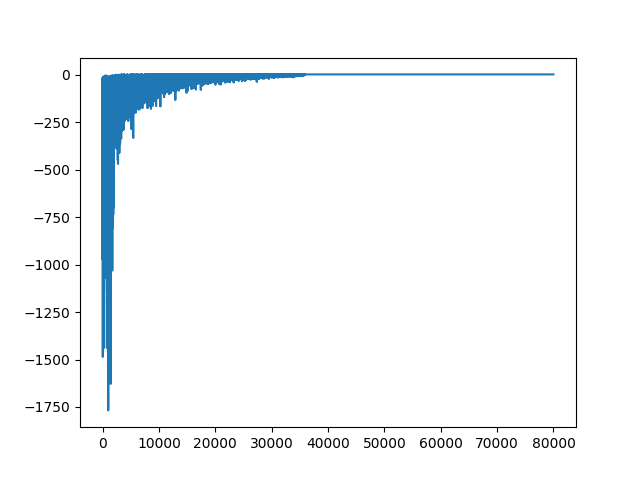
\includegraphics[width=30em]{img/esempio_plot.png}
	\caption{Esempio di grafico ottenuto dopo la fase di training (80000 epoche, 1500 step). Sull'asse x il numero di epoche, sull'asse y il reward totale per epoca.}
\end{figure}

Dal precedente grafico possiamo notare come nel primo periodo di tempo (da 0 a 40000 epoche) vi \`{e} la fase di \textit{exploration}, in quanto l'agente sta esplorando il labirinto con azioni casuali (molte di queste comportano l'impatto contro un muro, perci\`{o} inizialmente il reward totale \`{e} estremamente basso), successivamente (da 40000 a 80000 epoche) possiamo notare come l'agente \`{e} riuscito a trovare la via di fuga e converge sempre alla soluzione passando quindi alla fase di \textit{exploitation}.\\

\begin{minipage}{\linewidth}
\begin{lstlisting}[style=python]
def training(self, epochs=50000, steps=200, ALPHA=0.1, GAMMA=1.0, EPS=1.0):
	# inizializza la matrice Q
	Q = {}
	for state in self.env.stateSpace:
		for action in self.env.possibleActions:
			Q[state, action] = 0

	self.env.reset()
	self.env.render(gui=False)

	totalRewards = np.zeros(epochs)
	for i in range(epochs):
		if i % int(epochs / 10) == 0:
			print('starting game ', i)

		done = False
		epRewards = 0
		numActions = 0
		observation = self.env.reset()
		while not done and numActions <= steps:
			rand = np.random.random()
			
			if rand < (1 - EPS):
				action = self.maxAction(Q, observation, self.env.possibleActions)
			else:
				action = self.env.actionSpaceSample()

			observationNext, reward, done, info = self.env.step(action)
			numActions += 1
			epRewards += reward
			actionNext = self.maxAction(Q,observationNext,self.env.possibleActions)
			Q[observation, action] = Q[observation, action] + ALPHA * (reward +
													GAMMA * Q[observationNext, actionNext] - 
															Q[observation, action])
				observation = observationNext

		# permettere il cambio tra exploration ed exploitation
		if EPS - 2 / epochs > 0:
			EPS -= 2 / epochs
		else:
			EPS = 0

		totalRewards[i] = epRewards

	if plot:
		plt.plot(totalRewards)
		plt.show()
		
	self.saveQ(Q, "Qmatrix")
	
\end{lstlisting}
\end{minipage}

\subsubsection{execute}

\begin{lstlisting}[style=python, caption={Parte di codice del metodo execute}]
def execute(self,step_by_step=False,sleep_time=0.5,maxk=30,gui=True): -> bool
	self.env.reset()
	self.env.render(gui=gui)
	Q = self.loadQ("Qmatrix")
	...
	# esecuzione automatica
	totReward = 0
	alive = True
	action_counter = 0
	while action_counter < maxk:
		action = self.maxAction(
			Q,
			self.env.state_to_int(self.env.moore()),
			self.env.possibleActions
		)

		observationNext, reward, done, info = self.env.step(action)
		totReward += reward
		action_counter += 1
		
		print(f"Action: {action} Reward: {reward}\n")
		self.env.render(gui=gui)
		
		if done:
			print(f"Return: {totReward}")
			return True

		sleep(sleep_time)  # tempo di attesa per visualizzare lo stato successivo
		system("clear")

	return False
	
\end{lstlisting}
\ \\
Il metodo \lstinline[style=cmd]|execute| gestisce la fase di \textit{testing/execution} permettendo di visualizzare a schermo il comportamento dell'agente in un dato labirinto. La parte pi\`{u} interessante di questa funzione \`{e} quella riportata sopra: possiamo notare come inizialmente viene preparato l'ambente (righe 1 - 4) e caricata la \textit{matrice Q} per poi passare alla fase di esecuzione vera e propria (righe 10 - 30). Qui notiamo come ad ogni iterazione viene scelta la miglior mossa (vedi \autoref{sec:maxaction}) da effettuare nello stato attuale (righe 11 - 15), la quale viene eseguita ottenendo l'osservazione e il reward (riga 17) dall'ambiente, viene mostrata a video (riga 22) ed infine si controlla se l'agente \`{e} arrivato allo stato goal e nel caso, l'esecuzione viene interrotta (righe 23 - 25). Possiamo notare come l'agente ha a disposizione un massimo di \lstinline[style=cmd]|maxk| azioni per trovare l'uscita, dopo le quali l'esplorazione terminer\`{a} e verr\`{a} considerata come fallita (riga 10). Questo metodo ritorna \lstinline[style=cmd]|True| se l'agente \`{e} riuscito a trovare la via di fuga, altrimenti \lstinline[style=cmd]|False|.\\

La rappresentazione della mossa pu\`{o} essere di due tipi: \textbf{CLI} o \textbf{GUI}.\\
Nel primo caso verr\`{a} stampata la matrice nel terminale, nell'altro una finestra di \lstinline[style=cmd]|pygame| verr\`{a} mostrata. Di seguito un esempio:

\begin{figure}[H]
	\centering
	\begin{subfigure}{.5\textwidth}
		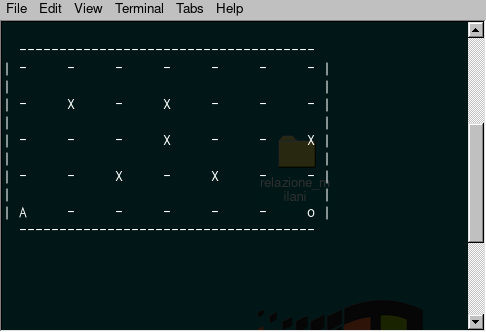
\includegraphics[width=.9\linewidth]{img/maze_cli.png}
	\end{subfigure}%
	\begin{subfigure}{.5\textwidth}
		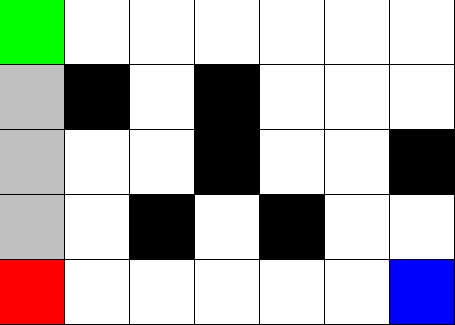
\includegraphics[width=.9\linewidth]{img/maze_gui.png}
	\end{subfigure}%
	\caption{Esempio di otuput CLI (a sinistra) e GUI (a destra) della stessa matrice con 4 azioni \lstinline[style=cmd]|D|}
\end{figure}


\subsubsection{maxAction}
\label{sec:maxaction}

Questo metodo si occupa di scegliere la migliore azione da compiere in base alla posizione dell'agente (riga 3). Questa scelta viene effettuata trovando il massimo tra i valori della riga (della \textit{matrice Q}) relativa allo stato attuale in cui l'agente si trova (vedi \autoref{sec:matriceQ}).\\

\begin{lstlisting}[style=python, caption={Codice del metodo maxAction}]
def maxAction(self, Q, state, actions: list[str]) -> str:
	values = np.array([Q[state, a] for a in actions])
	action = np.argmax(values)

	return actions[action]
	
\end{lstlisting}

\subsection{GUI.py}

All'interno di questo file risiede la classe che si occupa della stampa a video dei labirinti. Non andremo ad analizzare il codice ma vedremo solo come vengono rappresentati e cosa indica ogni elemento.

\subsubsection{CLI}

Questa modalit\`{a} di stampa mostra la matrice nel terminale. Gli elementi che compongono questo tipo di rappresentazione sono:

\begin{itemize}
	\item \lstinline[style=cmd]| - |: indica uno spazio vuoto e percorribile dall'agente (da non confondersi con la cinta di mura che delimita il labirinto)
	\item \lstinline[style=cmd]|X|: indica un muro
	\item \lstinline[style=cmd]|A|: indica dove si trova l'agente
	\item \lstinline[style=cmd]|o|: indica l'uscita del labirinto
	\item \lstinline[style=cmd]|------|: cinta di mura superiore ed inferiore che delimita il labirinto
	\item $|$: cinta di mura laterali che delimitano il labirinto
\end{itemize}

\begin{figure}[H]
	\centering
	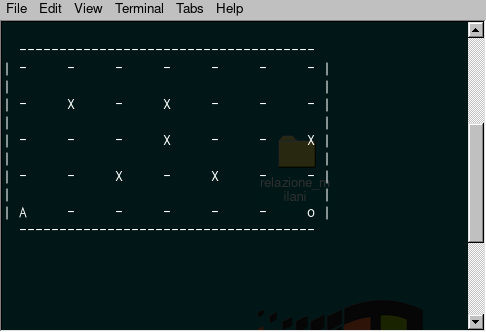
\includegraphics[width=.5\textwidth]{img/maze_cli.png}
	\caption{Esempio di rappresentazione CLI di un labirinto.}
\end{figure}

\subsubsection{GUI}

Questo tipo di stampa mostra a schermo una finestra di \lstinline[style=cmd]|pygmae| con all'interno una griglia che rappresenta il labirinto. Ogni cella ha un diverso colore che sta ad indicare:

\begin{itemize}
	\item verde (\crule[green]{.5em}{.5em}): la posizione di partenza dell'agente
	\item rosso (\crule[red]{.5em}{.5em}): la posizione attuale dell'agente
	\item bianco (\crule[white]{.5em}{.5em}): una cella vuota 
	\item blu (\crule[blue]{.5em}{.5em}): l'uscita del labirinto
	\item grigio (\crule[lightgray]{.5em}{.5em}): il cammino effettuato dall'agente
	\item nero (\crule{.5em}{.5em}): un muro
\end{itemize}

\begin{figure}[H]
	\centering
	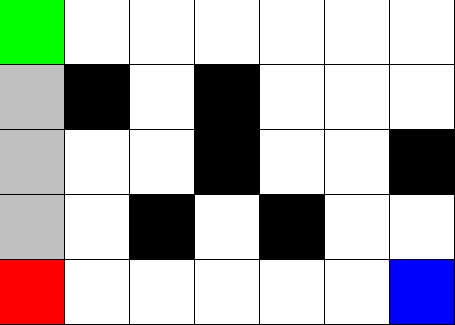
\includegraphics[width=.3\textwidth]{img/maze_gui.png}
	\caption{Esempio di rappresentazione GUI di un labirinto.}
\end{figure}

\subsection{training.py}
\label{sec:training}

In questo script \`{e} presente la funzione che permette all'utente di scegliere i parametri di \textit{training} e dare inizio all'allenamento. \`{E} possibile allenare l'agente utilizzando una sola matrice definita dall'utente o utilizzare l'intero dataset di training. C'\`{e} la possibilit\`{a} di iniziare un nuovo allenamento (andando a ricreare la matrice Q) o riprenderne uno gi\`{a} avviato in precedenza (andando a caricare una matrice Q gi\`{a} esistente).

\begin{lstlisting}[style=python, caption={Parte di codice della funzione che avvia la fase di allenamento utilizzando il dataset creato in precedenza}]
...
print(f"Avvio training sul dataset: {dataset}")

QL = QLearning(None)

# ottengo tutti i file nella cartella del dataset
filenames = next(walk(dataset), (None, None, []))[2]
for file in filenames:
	grid, message = grid_from_file(f"{dataset}/{file}")

	if grid is None:
		print(f"Errore in {file}: {message}")

	print(f"Caricato labirinto {grid.shape}")

	env = MazeEnv(grid=grid)
	QL.env = env
	QL.training(
			epochs=epochs, steps=steps, 
			ALPHA=alpha, GAMMA=gamma, EPS=eps, 
			plot=False, resume=resume, plot_name=file
	)
	
\end{lstlisting}
\pagebreak
\subsection{testing.py}
\label{sec:testing}

Qui risiede la funzione per avviare la fase di \textit{testing/execution} facendo scegliere all'utente i vari parametri come: avviare la modalit\`{a} \lstinline[style=cmd]|step-by-step| o quella automatica, se testare l'agente su un labirinto definito dall'utente o su tutti quelli presenti nel dataset di testing, ecc. Una funzione degna di nota \`{e} \lstinline[style=cmd]|evaluate()| che permette di "stimare" la precisione dell'agente in un modo abbastanza rudimentale:

\begin{itemize}
	\item Testa l'agente su ogni labirinto nel dataset di testing.
	\item Conta quanti labirinti l'agente \`{e} stato in grado di risolvere
	\item Calcola la precisione dell'agente: $\sfrac{labirinti \ risolti}{labirinti \ totali}$
	\item Ripete questa procedura per 5 volte ottenendo una media finale
\end{itemize}

Questo indice permetter\`{a} in futuro di confrontare diversi allenamenti (differenti matrici Q) tra di loro e capire quindi qual \`{e} il migliore.\\

\begin{lstlisting}[style=python, caption={Funzione per la valutazione dell'apprendimento}]
def evaluate():
	def _evaluate():
		QL = QLearning(None)
		tot = 0
		rew = 0
		filenames = next(walk(dataset), (None, None, []))[2]
		for file in filenames:
			grid, message = grid_from_file(f"{dataset}/{file}")
			env = MazeEnv(grid=grid)
			QL.env = env
			
			result,reward = QL.execute(step_by_step=False,sleep_time=0.0,gui=False)
			tot += result
			rew += reward
		return tot/len(filenames), rew

	avg_acc = 0
	avg_rew = 0
	max_step = 5
	
	for _ in range(max_step):
		acc, rew = _evaluate()
		avg_acc += acc
		avg_rew += rew
	
	avg_acc /= max_step
	avg_rew /= max_step
	
	print(f"Acc avg: {avg_acc} Rew avg: {avg_rew}")
	
\end{lstlisting}

\section{Svolgimento}

In questa sezione andr\`{o} a descrivere i vari esperimenti, problemi e soluzioni, con anche parti di codice, che ho incontrato durante la realizzazione di questo progetto.

\subsection{Primo allenamento}
\label{sec:primoallenamento}

Come primo allenamento ho deciso di utilizzare un labirinto tra quelli presenti nel dataset di training. Ho scelto uno dei pi\`{u} grandi per permettere all'agente di esplorare uno spazio abbastanza ampio in modo da poter riempire pi\`{u} righe della matrice Q possibile. Ho scelto \lstinline[style=cmd]|matrice_69|, una $9 \times 9$ con una disposizione delle mura abbastanza complessa.

\begin{figure}[H]
	\centering
	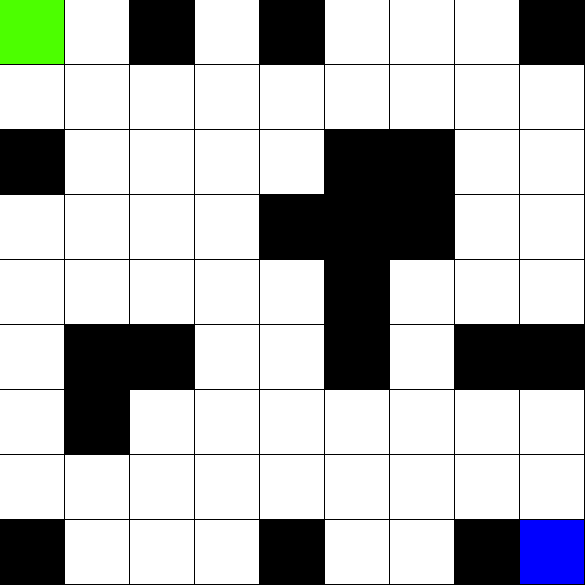
\includegraphics[width=.3\textwidth]{img/matrice_69.png}
	\caption{Rappresentazione grafica del labirinto scelto per il primo allenamento.}
\end{figure}

Ho quindi deciso di allenare l'agente con i seguenti parametri:

\begin{figure}[H]
	\centering
	\begin{tabular}{c | c | c | c | c}
		\textbf{Epoche}: 50k & \textbf{Step}: 400 & \textbf{Alpha}: 0.1 & \textbf{Gamma}: 1.0 & \textbf{EPS}: 0.9
	\end{tabular}
\end{figure}
\begin{figure}[H]
	\centering
	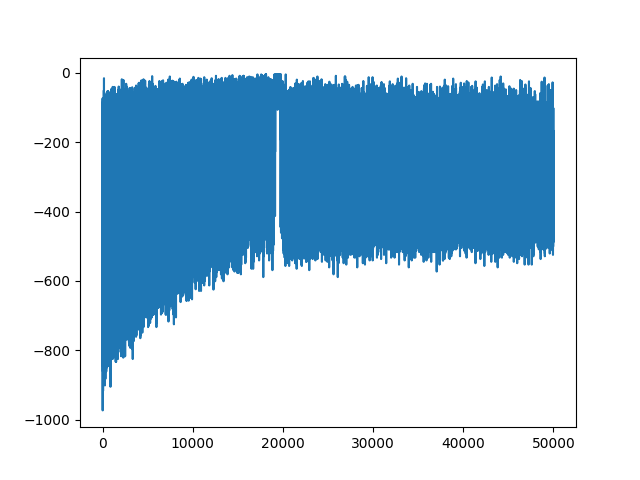
\includegraphics[width=.6\textwidth]{img/primo_allenamento.png}
	\caption{Grafico del risultato del primo allenamento.}
\end{figure}

Dal grafico sopra mostrato \`{e} evidente che l'agente non \`{e} riuscito a trovare l'uscita per via dell'insufficiente numero di step ed epoche utilizzato. Anche dalla fase di esecuzione,  utilizzando sia la stessa matrice della fase di training che una mai esplorata, si vede chiaramente che l'agente non \`{e} in grado di uscire dal labirinto. Nel primo caso l'agente rimane bloccato in un loop di azioni infinito (\lstinline[style=cmd]|L| \lstinline[style=cmd]|R|), nel secondo impatta sempre contro un muro.

\begin{figure}[H]
	\centering
	\begin{subfigure}{.5\textwidth}
		\centering
		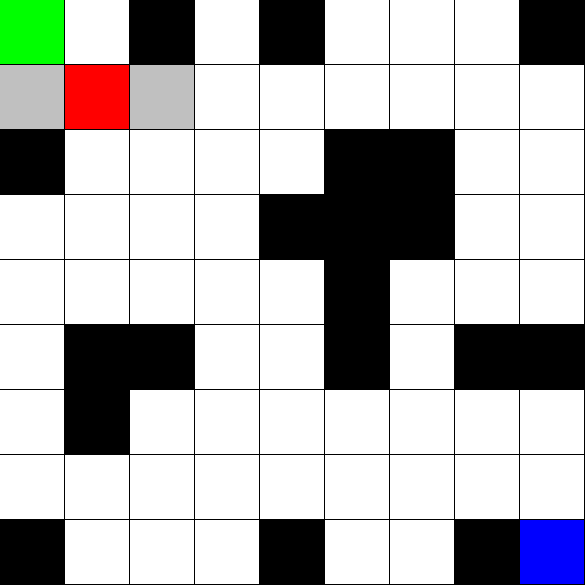
\includegraphics[width=.7\linewidth]{img/primo_allenamento_agente.png}
	\end{subfigure}%
	\begin{subfigure}{.5\textwidth}
		\centering
		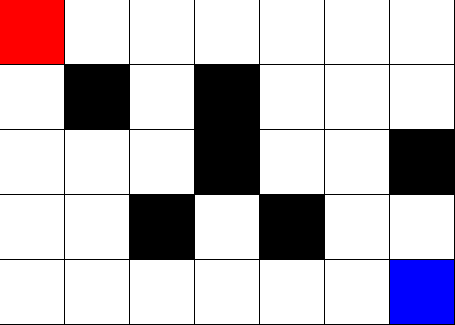
\includegraphics[width=.8\linewidth]{img/primo_allenamento_rotto.png}
	\end{subfigure}%
	\caption{A sinistra l'agente rimane bloccato tra due azioni, a destra l'agente impatta sempre contro il muro.}
\end{figure}

Inoltre, analizzando meglio la \textit{matrice Q} ed il codice in \lstinline[style=cmd]|QLearning.py| sorge un ulteriore problema: quando l'agente si trova un uno stato mai visto esegue sempre la prima azione (\lstinline[style=cmd]|U|)! Questo per via da della riga 3 della funzione \lstinline[style=cmd]|maxAction| (vedi \autoref{sec:maxaction}), \lstinline[style=cmd]|np.argmax()| sceglie il massimo tra gli elementi in input e nel caso ce ne fossero 2 o pi\`{u} uguali, prende sempre il primo che trova.

\subsubsection{Problema 1: convergenza}
\label{sec:problema1}

Per un labirinto $9 \times 9$, 50000 epoche e 400 step non sono sufficienti per trovare la soluzione (vedi \autoref{sec:primoallenamento}). Dato che il dataset di training contiene matrici grandi al massimo $10 \times 10$ potrebbe compromettere il risultato della fase di allenamento.

\subsubsection{Soluzione a \hyperref[sec:problema1]{Problema 1}}
\label{sec:solprob1}

Per risolvere questo problema procedo a tentativi nel seguente modo:

\begin{enumerate}
	\item Provo ad \textit{aumentare} il numero di \textit{epoche} tenendo \textit{costante} il numero di \textit{step}.
	\item Provo ad \textit{aumentare} il numero di \textit{step} tenendo \textit{costante} il numero di \textit{epoche}.
	\item Provo ad \textit{aumentare} sia il numero di \textit{epoche} che il numero di \textit{step}.
\end{enumerate}

\begin{figure}[H]
	% 60000 400		|	50000 450		|	60000 450
	% 70000 400		|	50000 600		|	70000 600
	% 80000 400		|	50000 1000	   |	80000 1000
	\begin{subfigure}{\textwidth}
		\centering
		\begin{subfigure}{.33\textwidth}
			\centering
			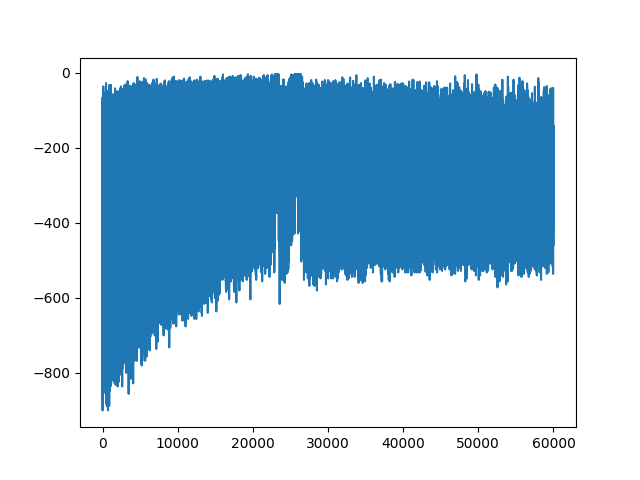
\includegraphics[width=1\linewidth]{img/plot_60k_400.png}
			\caption{60k epoche, 400 step}
		\end{subfigure}%
		\begin{subfigure}{.33\textwidth}
			\centering
			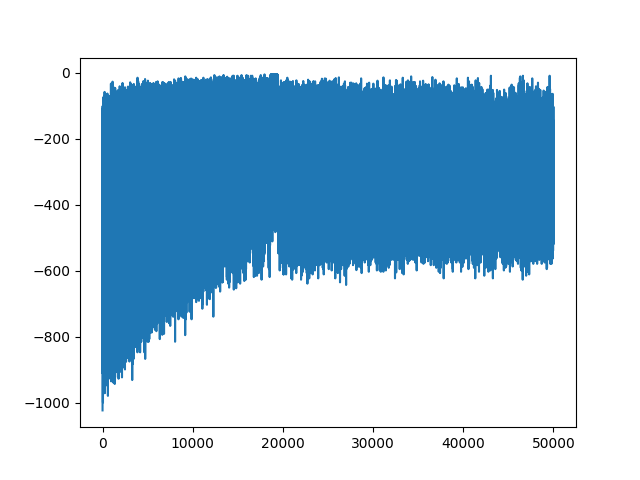
\includegraphics[width=1\linewidth]{img/plot_50k_450.png}
			\caption{50k epoche, 450 step}
		\end{subfigure}%
		\begin{subfigure}{.33\textwidth}
			\centering
			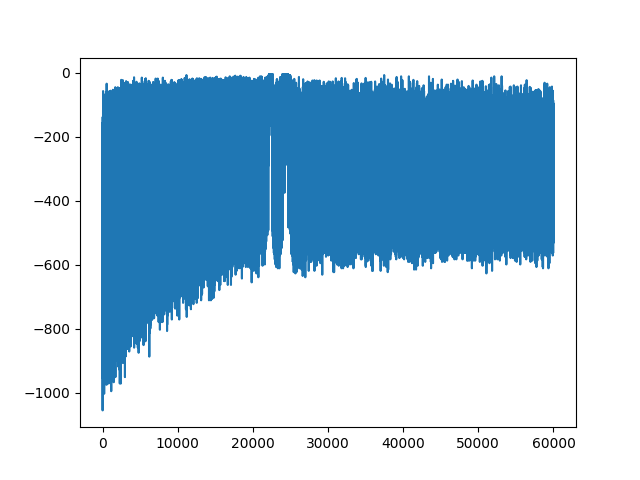
\includegraphics[width=1\linewidth]{img/plot_60k_450.png}
			\caption{60k epoche, 450 step}
		\end{subfigure}%
	\end{subfigure}
	\begin{subfigure}{\textwidth}
		\centering
		\begin{subfigure}{.33\textwidth}
			\centering
			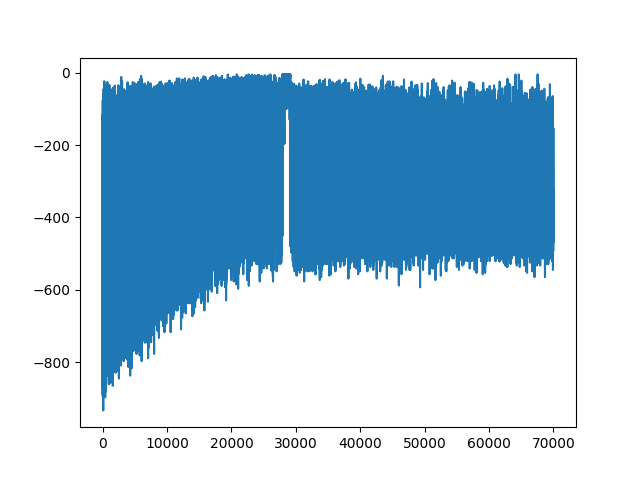
\includegraphics[width=1\linewidth]{img/plot_70k_400.png}
			\caption{70k epoche, 400 step}
		\end{subfigure}%
		\begin{subfigure}{.33\textwidth}
			\centering
			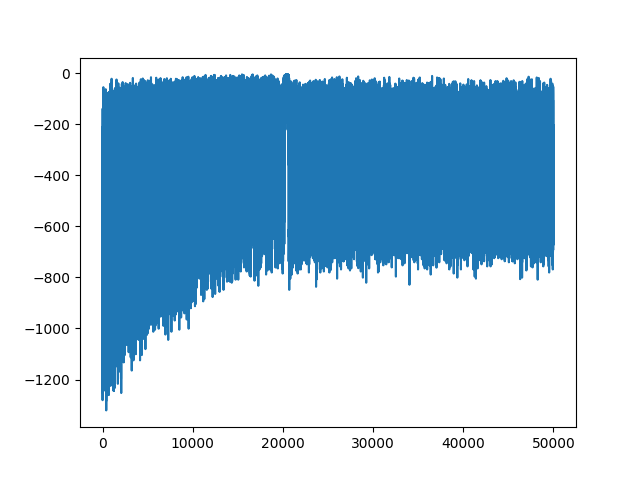
\includegraphics[width=1\linewidth]{img/plot_50k_600_cattivo.png}
			\caption{50k epoche, 600 step}
		\end{subfigure}%
		\begin{subfigure}{.33\textwidth}
			\centering
			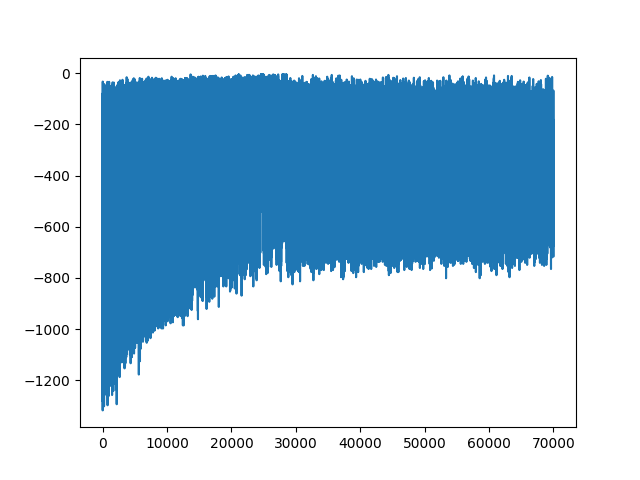
\includegraphics[width=1\linewidth]{img/plot_70k_600.png}
			\caption{70k epoche, 600 step}
		\end{subfigure}%
	\end{subfigure}
	\begin{subfigure}{\textwidth}
		\centering
		\begin{subfigure}{.33\textwidth}
			\centering
			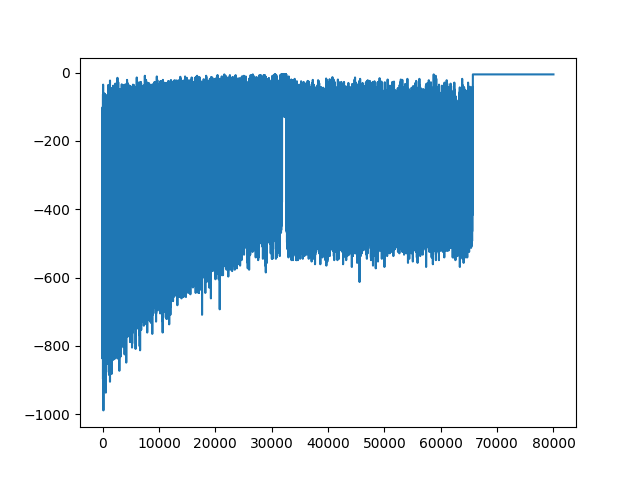
\includegraphics[width=1\linewidth]{img/plot_80k_400.png}
			\caption{80k epoche, 400 step}
		\end{subfigure}%
		\begin{subfigure}{.33\textwidth}
			\centering
			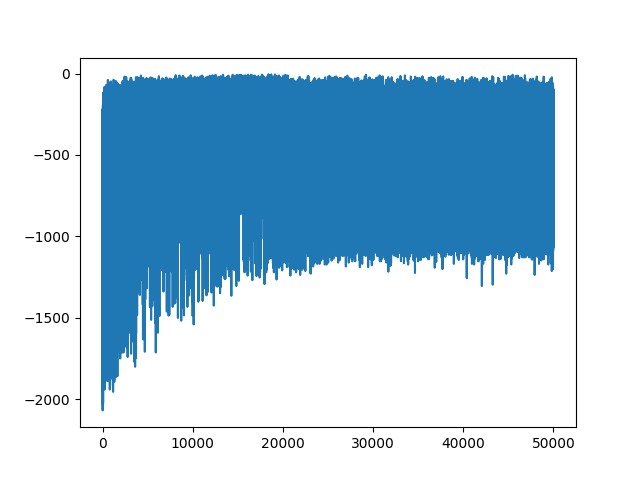
\includegraphics[width=1\linewidth]{img/plot_50k_1000.png}
			\caption{50k epoche, 1000 step}
		\end{subfigure}%
		\begin{subfigure}{.33\textwidth}
			\centering
			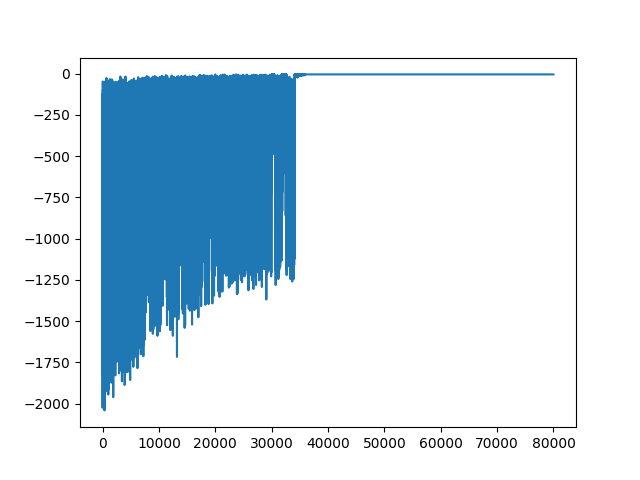
\includegraphics[width=1\linewidth]{img/plot_80k_1000(2).png}
			\caption{80k epoche, 1000 step}
		\end{subfigure}%
	\end{subfigure}
	\caption{Confronto tra training sulla stessa matrice con epoche e step differenti.}
\end{figure}

Dai grafici mostrati in precedenza si nota che solo in 2 casi l'agente \`{e} riuscito a trovare la soluzione: (g) e (i). Nel caso di (g), si vede come solo vero l'ultima parte della fase di allenamento, l'agente sia riuscito a trovare una soluzione, invece in (i), ha si esplorato inizialmente, ma ha trovato l'uscita decisamente prima. Hanno anche tempi di esecuzione e reward totali differenti, come possiamo notare dalla seguente tabella:

\begin{figure}[H]
	\centering
	\begin{tabular}{c | c | c}
		\textbf{Training} & \textbf{Tempo di esecuzione (minuti)} & \textbf{Reward Totale}\\
		\hline
		(g) & 14 : 52 . 40 \rule{0pt}{1.2em} & -7\\
		(i) & 08 : 34 . 95 & -5\\
	\end{tabular}
	\caption{Confronto trai tempi di esecuzione e reward dei 2 allenamenti.}
\end{figure}

Deduco quindi che (i) risulta essere la migliore combinazione di epoche e step avendo il minor tempo di esecuzione con il maggior reward totale.

\subsubsection{Problema 2: stato sconosciuto}
\label{sec:problema2}

L'agente quando si trova in uno stato sconosciuto andr\`{a} sempre ad eseguire l'azione \lstinline[style=cmd]|U| (vedi \autoref{sec:primoallenamento}).

\subsubsection{Soluzione a \hyperref[sec:problema2]{Problema 2}}
\label{sec:solprob2}

Per risolvere questo problema vado a modificare la funzione  \lstinline[style=cmd]|maxAction| (vedi \autoref{sec:maxaction}) facendo ritornare, solo se in fase di esecuzione, un'azione a caso qualora 2 o pi\`{u} elementi della riga presa in considerazione risultino uguali. Questo probabilmente andr\`{a} a "sbloccare" l'agente facendolo arrivare in uno stato a lui conosciuto, al costo di  eseguire mosse poco intelligenti (potrebbe andare a sbattere contro un muro) ed introdurre aleatoriet\`{a} nella fase di esecuzione.\\

\begin{figure}[H]
	\begin{equation*}
		\begin{bmatrix}
			0.000000 &  0.000000 & 0.000000 & 0.000000
		\end{bmatrix}
	\end{equation*}
	\caption{Esempio di stato mai visitato.}
\end{figure}

Se invece, l'agente \`{e} "indeciso" tra 2 mosse (solo 2 elementi della riga sono uguali), questa modifica risulter\`{a} decisamente pi\`{u} efficacie dato che sceglier\`{a} si un'azione casualmente, ma sar\`{a} un'azione sensata e valida che molto probabilmente lo condurr\`{a} in uno stato a lui noto.

\begin{figure}[H]
	\begin{equation*}
		\begin{bmatrix}
			0.000000 &  -1.405382 & 0.000000 & -5.872155
		\end{bmatrix}
	\end{equation*}
	\caption{Esempio di indecisione tra 2 mosse.}
\end{figure}

\begin{lstlisting}[style=python, caption={Modifica per risoluzione a Problema 2}]
def maxAction(self, Q, state, actions: list[str], in_execution=False) -> str:
	values = np.array([Q[state, a] for a in actions])
	action = np.argmax(values)

	# prende a caso un'azione se ce ne sono due o piu' uguali
	if in_execution:
		tmp = [i for i, x in enumerate(values) if x == values[action]]
		if len(tmp) > 1:
			action = np.random.choice(tmp)
			
	return actions[action]
	
\end{lstlisting}

\subsection{Secondo Allenamento}

Avendo applicato \hyperref[sec:solprob1]{Soluzione a Problema 1} e \hyperref[sec:solprob2]{Soluzione a Problema 2} effettuo un secondo allenamento, sempre sulla matrice scelta in \autoref{sec:primoallenamento} e con i seguenti parametri:

\begin{figure}[H]
	\centering
	\begin{tabular}{c | c | c | c | c}
		\textbf{Epoche}: 80k & \textbf{Step}: 1000 & \textbf{Alpha}: 0.1 & \textbf{Gamma}: 1.0 & \textbf{EPS}: 0.9\\
	\end{tabular}
\end{figure}

Successivamente vado prima a testarlo sul labirinto con cui \`{e} stato allenato, poi con una matrice mai vista, infine effettuo la valutazione come descritto in \autoref{sec:testing}.

\begin{figure}[H]
	\centering
	\begin{subfigure}[b]{.5\textwidth}
		\centering
		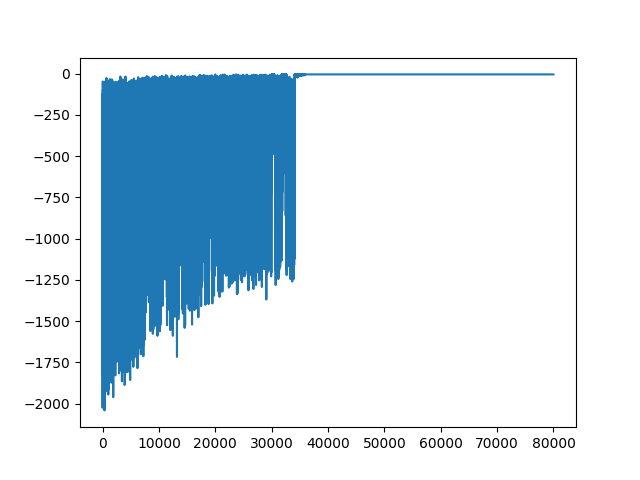
\includegraphics[width=\textwidth]{img/plot_80k_1000(2).png}
		\caption{Grafico di training}
	\end{subfigure}%
	\begin{subfigure}[b]{.5\textwidth}
		\centering
		\begin{figure}[H]
			\centering
			\begin{tabular}{c c c}
				\textbf{Acc (avg)}& \vline & \textbf{Rew (avg)}\\
				\hline
			    & \vline & \\ [.01em]
				0.12 & \vline & -1378.8 \\ [1.5em]
				& & \\ 
				&&  \\ 
				& & \\ 
			\end{tabular}
		\end{figure}
		\caption{Valutazione finale}
	\end{subfigure}%

	\ \\
	\begin{subfigure}[t]{.5\textwidth}
		\centering
		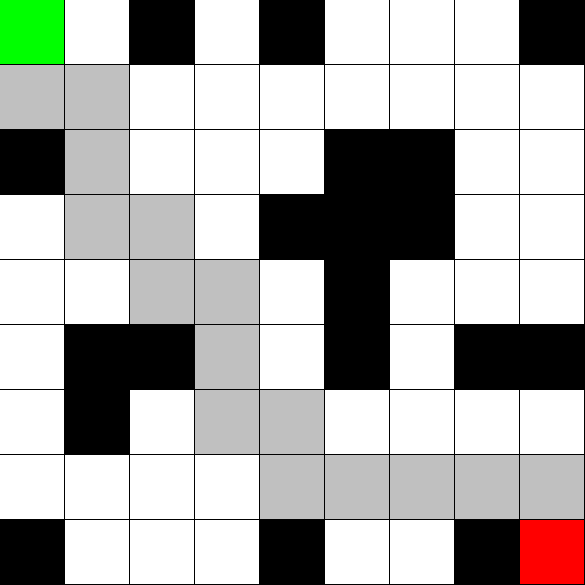
\includegraphics[width=0.6\textwidth]{img/secondo_train_success.png}
		\caption{L'agente nella matrice di training}
	\end{subfigure}%
	\begin{subfigure}[t]{.5\textwidth}
		\centering
		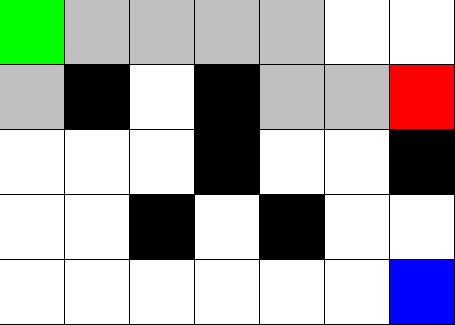
\includegraphics[width=.8\textwidth]{img/secondo_train_fail.png}
		\caption{L'agente in una matrice sconosciuta}
	\end{subfigure}%
	\caption{Risultati secondo allenamento}
\end{figure}

Dall'analisi dei risultati sopra mostrati, si pu\`{o} notare come l'agente risulta essere molto bravo a risolvere il labirinto su cui \`{e} stato allenato (c), ma appena viene messo all'interno di uno mai esplorato non sa come comportarsi: in (d) si vede come quest'ultimo sta procedendo in modo casuale sperando di arrivare, prima o poi, in una serie di stati conosciuti che lo porteranno al goal. Anche il risultato della valutazione generale (mostrata in (b)) \`{e} molto scadente: l'agente riesce, in media, a risolvere solo 2 labirinti tra i 20 presenti nel dataset di testing.%una media dei reward totali e della precisione estremamente bassa.
\pagebreak
\subsubsection{Problema 1}
\label{sec:problema11}

Il problema di questi scarsi risultati risiede nella matrice Q: moltissimi stati (in questo specifico caso 213) non sono mai stati esplorati e quindi l'agente sar\`{a} portato a scegliere azioni casuali invece che basarsi sulla "conoscenza" acquisita durante l'allenamento.\\

\begin{lstlisting}[style=python, basicstyle=\tiny, caption={Alcune righe della matrice Q}]
	-2.255275423663378547 -2.121039500176469517 -4.693440727996912032 -2.366805664424987867
	-2.374627887715270447 -2.373328666128976181 -2.372542805941218944 -2.372503147618498076
	0.0000000000000000000 0.0000000000000000000 0.0000000000000000000 0.0000000000000000000
	0.0000000000000000000 0.0000000000000000000 0.0000000000000000000 0.0000000000000000000
	-2.371282481079700517 -2.368817406376339818 -2.368644643610111871 -2.328848871442608868
	0.0000000000000000000 0.0000000000000000000 0.0000000000000000000 0.0000000000000000000
	0.0000000000000000000 0.0000000000000000000 0.0000000000000000000 0.0000000000000000000
	0.0000000000000000000 0.0000000000000000000 0.0000000000000000000 0.0000000000000000000
	0.0000000000000000000 0.0000000000000000000 0.0000000000000000000 0.0000000000000000000
	0.0000000000000000000 0.0000000000000000000 0.0000000000000000000 0.0000000000000000000
	0.0000000000000000000 0.0000000000000000000 0.0000000000000000000 0.0000000000000000000
	0.0000000000000000000 0.0000000000000000000 0.0000000000000000000 0.0000000000000000000
	0.0000000000000000000 0.0000000000000000000 0.0000000000000000000 0.0000000000000000000
\end{lstlisting}

Risulta quindi essere molto bravo nel trovare la fuga solo nella matrice con cui \`{e} stato allenato, negli altri labirinti non sa quasi mai come muoversi. In pratica la matrice Q \`{e} poco popolata.

\subsubsection{Soluzione a \hyperref[sec:problema11]{Problema 1}}
\label{sec:solprob11}

La soluzione a questo problema \`{e} abbastanza intuitiva: cercare di "mostrare" all'agente il maggior numero di stati possibili, in modo tale da accrescere la sua "esperienza". Ci\`{o} equivale a dire: popolare pi\`{u} righe possibili della matrice Q.\\

Allener\`{o} quindi l'agente utilizzando tutto il dataset di training (vedi \autoref{sec:progetto}, \autoref{sec:training}) con i seguenti parametri:

\begin{figure}[H]
	\centering
	\begin{tabular}{c | c | c | c | c}
		\textbf{Epoche}: 80k & \textbf{Step}: 1500 & \textbf{Alpha}: 0.1 & \textbf{Gamma}: 1.0 & \textbf{EPS}: 0.9\\
	\end{tabular}
\end{figure}

Per poi valutare i risultati e confrontarli con quelli ottenuti dall'allenameto precedente.

\subsection{Terzo allenamento}
\label{sec:terzo}

 Procedo quindi come descritto in \hyperref[sec:solprob11]{Soluzione a Problema 1}. Questo allenamento \`{e} risultato estremamente oneroso in termini di tempo: circa 6 ore. Dovendo analizzare cos\`{i} tante matrici, di dimensioni abbastanza elevate, \`{e} normale che questa fase sia molto lunga. Questo costo elevato \`{e} anche dato dall'impiego di un'architettura single thread durante la fase di allenamento. Il passaggio al multi threading appare effettivamente molto difficile in quanto ogni epoca dipende dall'esperienza appresa nell'epoca passata, in pi\`{u}, va implementata una gestione efficiente e sincronizzata della matrice Q.

\begin{figure}[H]
	\centering
	\begin{subfigure}{.25\textwidth}
		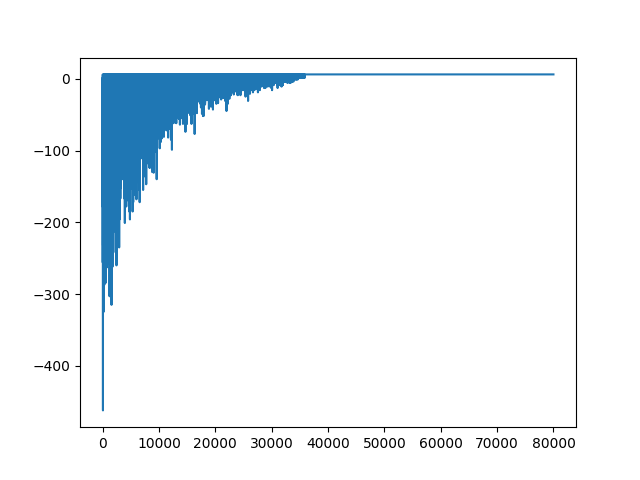
\includegraphics[width=\textwidth]{img/train/matrice_0-11_17_55.png}
	\end{subfigure}%
	\begin{subfigure}{.25\textwidth}
		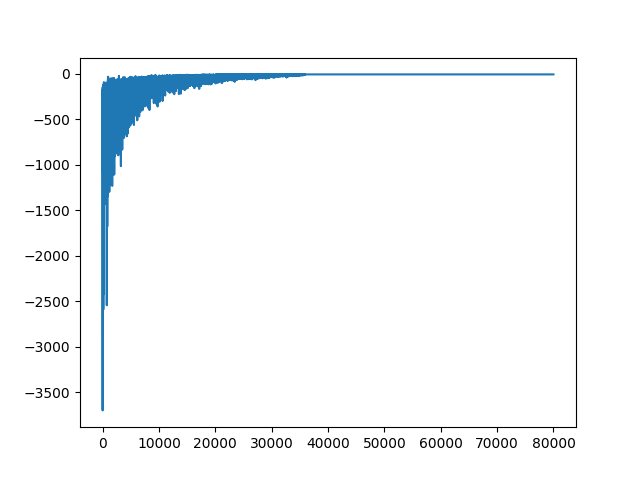
\includegraphics[width=\textwidth]{img/train/matrice_1-11_20_36.png}
	\end{subfigure}%
		\begin{subfigure}{.25\textwidth}
		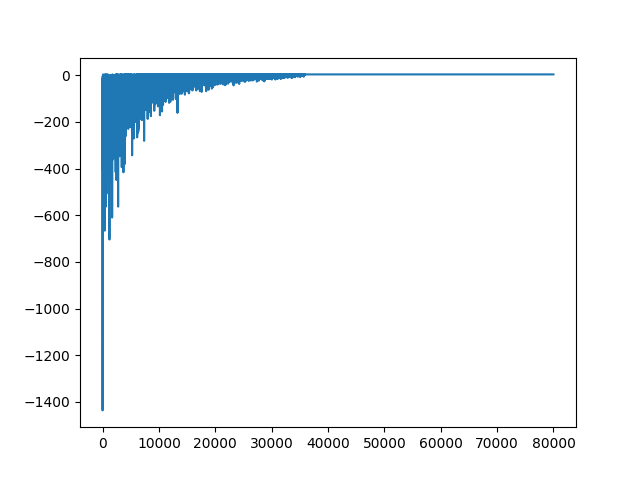
\includegraphics[width=\textwidth]{img/train/matrice_2-11_21_33.png}
	\end{subfigure}%
		\begin{subfigure}{.25\textwidth}
		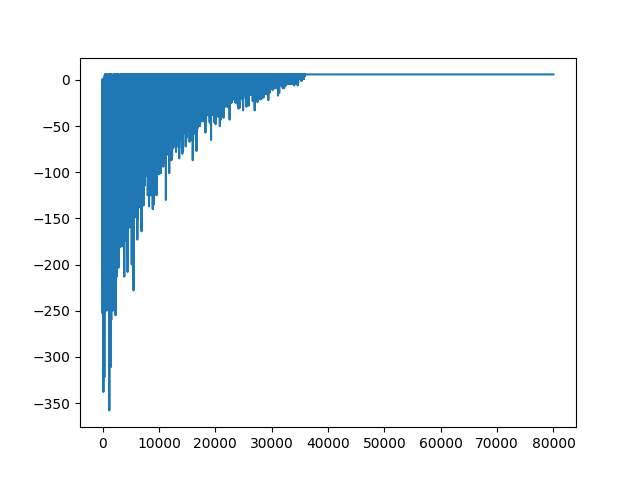
\includegraphics[width=\textwidth]{img/train/matrice_3-11_22_11.png}
	\end{subfigure}%

	\begin{subfigure}{.25\textwidth}
		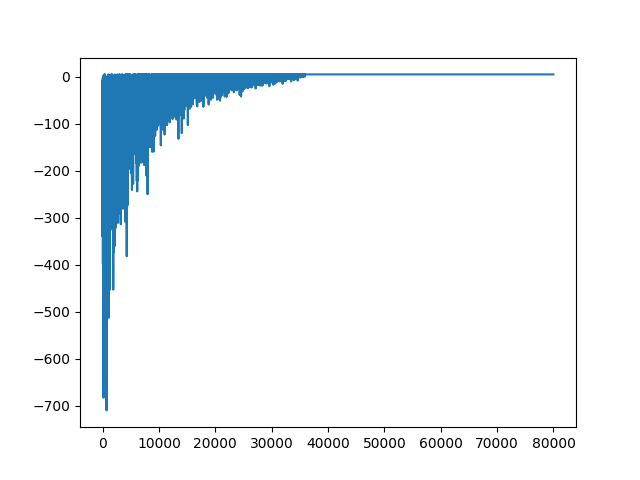
\includegraphics[width=\textwidth]{img/train/matrice_4-11_23_01.png}
	\end{subfigure}%
	\begin{subfigure}{.25\textwidth}
		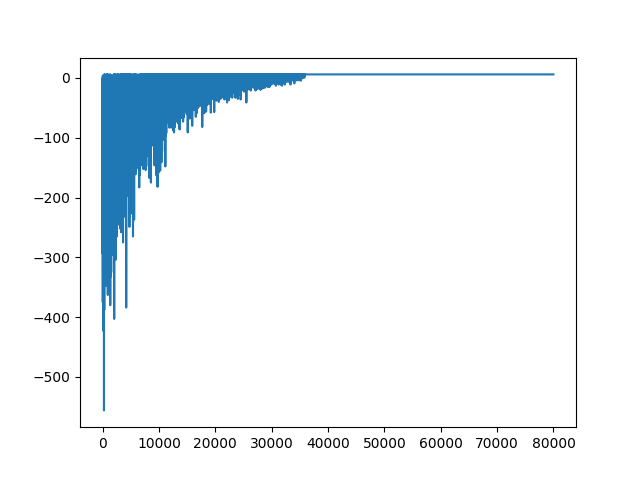
\includegraphics[width=\textwidth]{img/train/matrice_5-11_23_42.png}
	\end{subfigure}%
	\begin{subfigure}{.25\textwidth}
		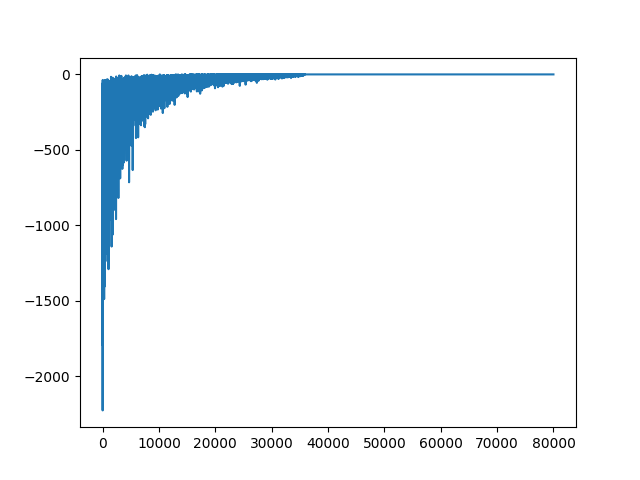
\includegraphics[width=\textwidth]{img/train/matrice_6-11_25_34.png}
	\end{subfigure}%
	\begin{subfigure}{.25\textwidth}
		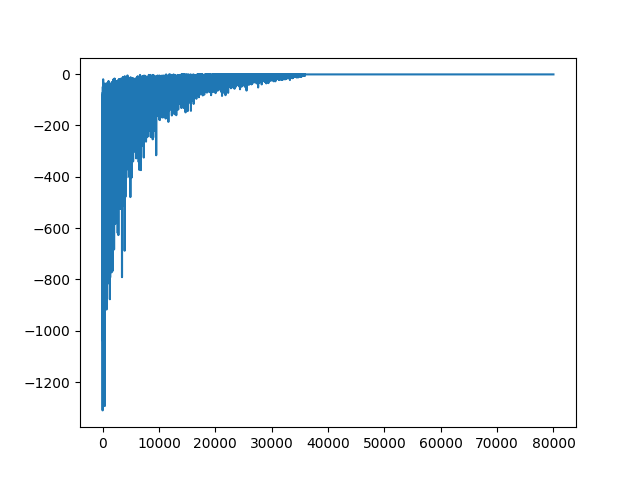
\includegraphics[width=\textwidth]{img/train/matrice_7-11_27_26.png}
	\end{subfigure}%
	
	\begin{subfigure}{.25\textwidth}
		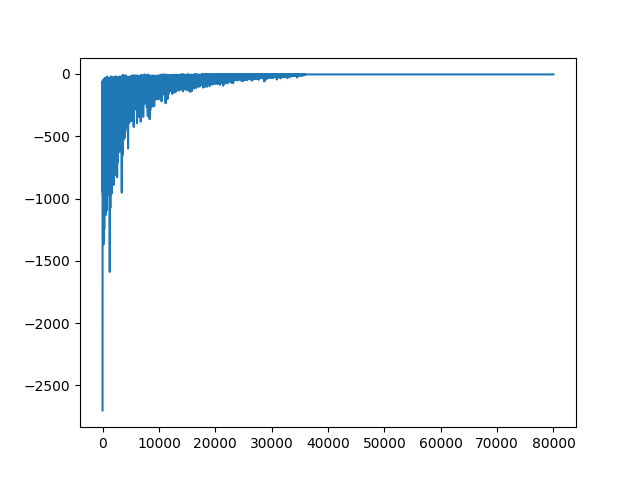
\includegraphics[width=\textwidth]{img/train/matrice_8-11_29_37.png}
	\end{subfigure}%
	\begin{subfigure}{.25\textwidth}
		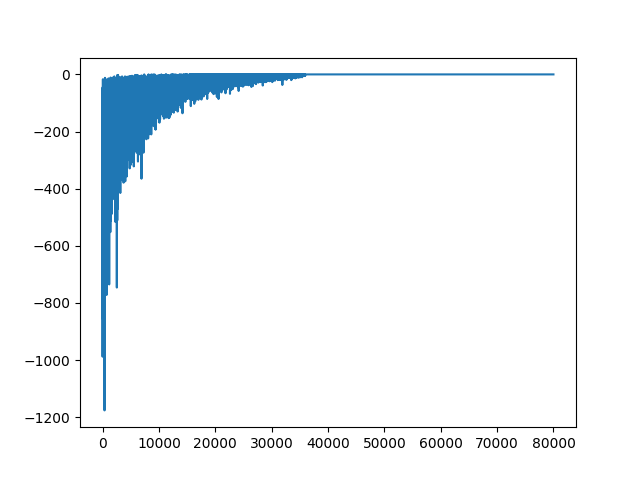
\includegraphics[width=\textwidth]{img/train/matrice_9-11_31_10.png}
	\end{subfigure}%
	\begin{subfigure}{.25\textwidth}
		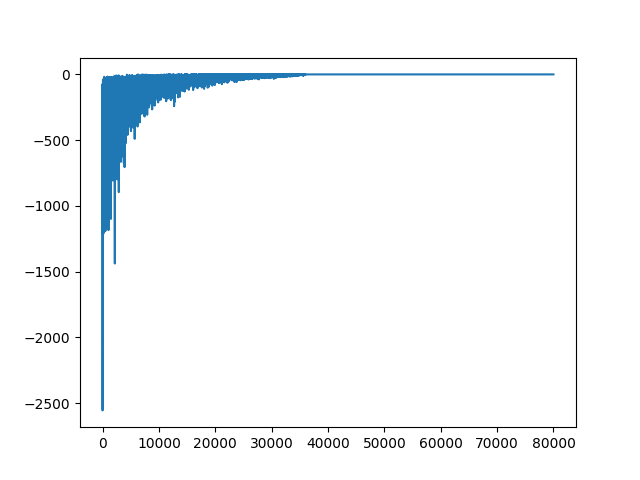
\includegraphics[width=\textwidth]{img/train/matrice_10-11_33_11.png}
	\end{subfigure}%
	\begin{subfigure}{.25\textwidth}
		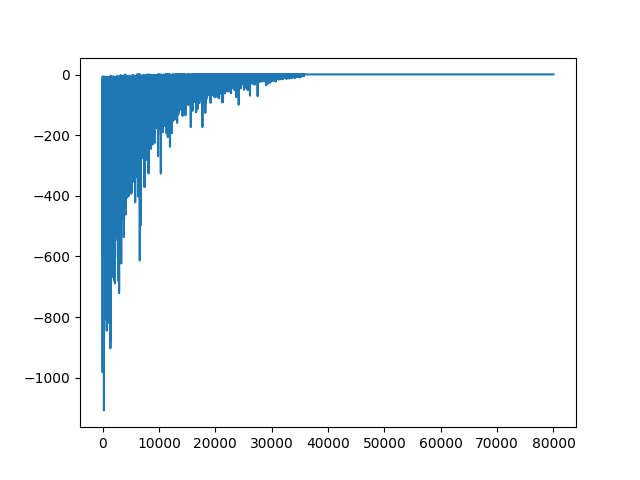
\includegraphics[width=\textwidth]{img/train/matrice_11-11_34_52.png}
	\end{subfigure}%

	\begin{subfigure}{.25\textwidth}
		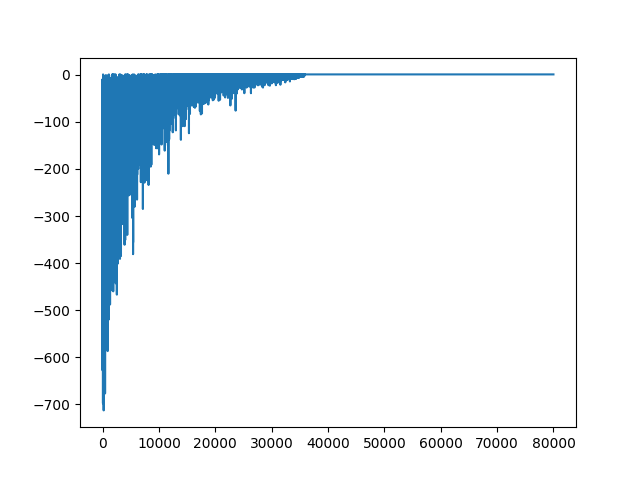
\includegraphics[width=\textwidth]{img/train/matrice_12-11_36_20.png}
	\end{subfigure}%
	\begin{subfigure}{.25\textwidth}
		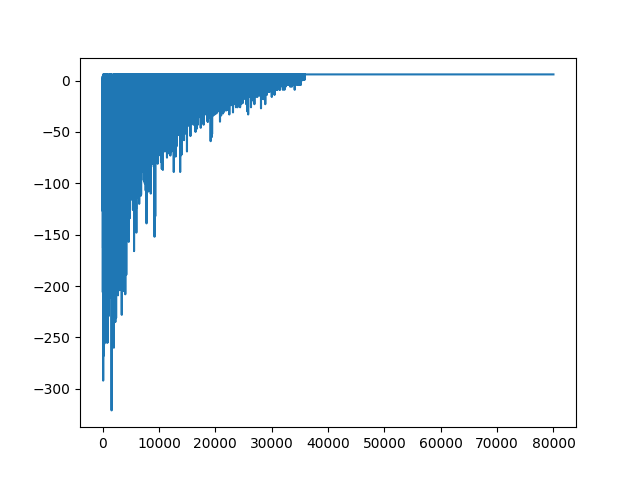
\includegraphics[width=\textwidth]{img/train/matrice_13-11_36_56.png}
	\end{subfigure}%
	\begin{subfigure}{.25\textwidth}
		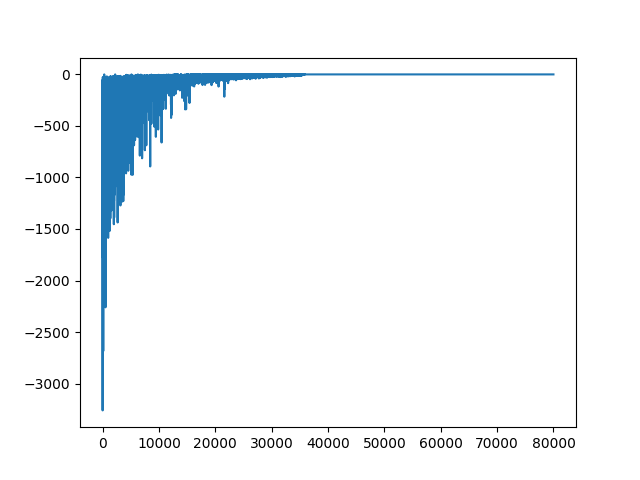
\includegraphics[width=\textwidth]{img/train/matrice_14-11_39_06.png}
	\end{subfigure}%
	\begin{subfigure}{.25\textwidth}
		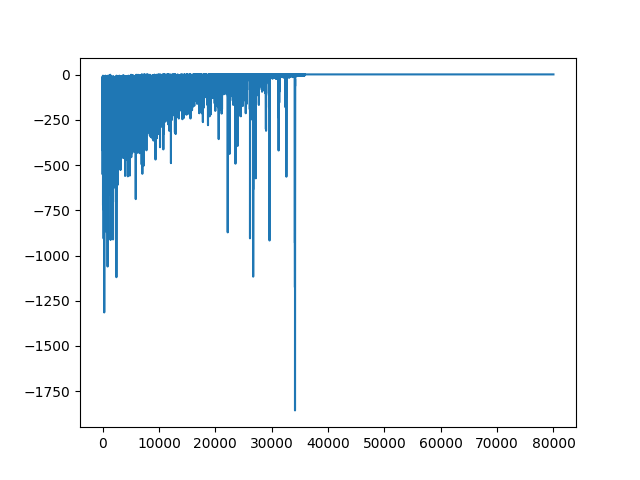
\includegraphics[width=\textwidth]{img/train/matrice_15-11_40_48.png}
	\end{subfigure}%
	
	\begin{subfigure}{.25\textwidth}
		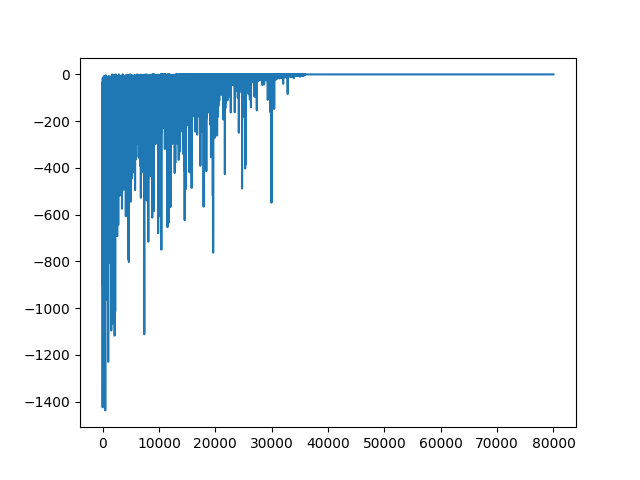
\includegraphics[width=\textwidth]{img/train/matrice_16-11_42_34.png}
	\end{subfigure}%
	\begin{subfigure}{.25\textwidth}
		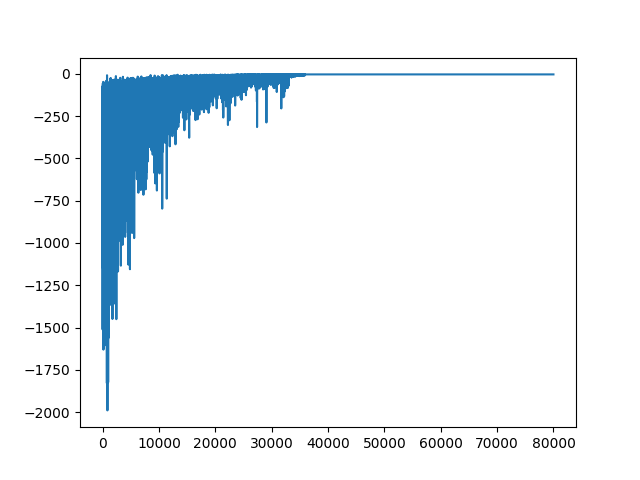
\includegraphics[width=\textwidth]{img/train/matrice_17-11_45_40.png}
	\end{subfigure}%
	\begin{subfigure}{.25\textwidth}
		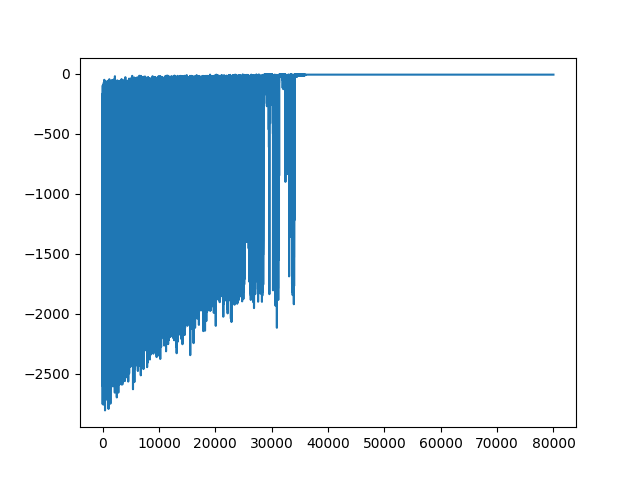
\includegraphics[width=\textwidth]{img/train/matrice_18-11_57_31.png}
	\end{subfigure}%
	\begin{subfigure}{.25\textwidth}
		\includegraphics[width=\textwidth]{img/train/matrice_19-12_02_37.png}
	\end{subfigure}%
	\caption{Alcuni dei grafici ottenuti durante la fase di training}
\end{figure}

\begin{figure}[H]
	\begin{subfigure}[b]{.5\textwidth}
		\centering
		\includegraphics[width=.7\textwidth]{img/terzo_success.png}
		\caption{L'agente in  una matrice mai vista}
	\end{subfigure}%
	\begin{subfigure}[b]{.5\textwidth}
	\centering
	\begin{figure}[H]
		\centering
		\begin{tabular}{c c c}
			\textbf{Acc (avg)}& \vline & \textbf{Rew (avg)}\\
			\hline
			& \vline & \\ [.01em]
			0.4 & \vline & -338.8 \\ [1.5em]
			& & \\ 
		\end{tabular}
	\end{figure}
	\caption{Valutazione finale}
\end{subfigure}%
\end{figure}

Dai dati sopra riportati possiamo notare come l'agente ora \`{e} in grado di risolvere una matrice mai vista prima (a) ed i valori medi di \textit{accuracy} e \textit{reward totale} sono migliorati notevolmente. Da un confronto pi\`{u} accurato possiamo notare che l'accuracy media \`{e} migliorata del 200\% circa e il reward totale medio del 300\%  circa. L'agente ora \`{e} in grado di uscire da quasi la met\`{a} dei labirinti presenti nel dataset di training contro solo i 2 precedenti !

\begin{figure}[H]
	\centering
	\begin{tabular}{c | c | c | c}
		& \textbf{Secondo Allenamento} & \textbf{Terzo Allenamento} &  \rule{0pt}{2em}\\ [1.4em]
		\hline
		\textbf{Accracy (avg)} & 0.12 & 0.4 \rule{0pt}{2em} & $\sim +200\%$ \\ [2em]
		\hline
		\textbf{Reward (avg) }& -1378.8 & -338.8 \rule{0pt}{2em}  & $\sim +300\%$ \\ [2em]
	\end{tabular}
\caption{Confronto tra Secondo Allenamento e Terzo Allenamento}
\end{figure}

Mettendo a confronto le due matrici Q possiamo vedere come quella attuale risulta decisamente pi\`{u} completa (e quindi migliore) della precedente in quanto solo 41 stati sono inesplorati (righe vuote) contro i 213 precedenti.\\

\begin{minipage}{\textwidth}
	\begin{minipage}{.45\textwidth}
		\begin{lstlisting}[style=python, basicstyle=\tiny, caption={Alcune righe della matrice Q di Secondo Allenamento}]
 -2.25527542 -2.12103950 -4.69344072 -2.36680566
 -2.37462788 -2.37332866 -2.37254280 -2.37250314
 0.000000000 0.000000000 0.000000000 0.000000000
 0.000000000 0.000000000 0.000000000 0.000000000
 -2.37128248 -2.36881740 -2.36864464 -2.32884887
 0.000000000 0.000000000 0.000000000 0.000000000
 0.000000000 0.000000000 0.000000000 0.000000000
 0.000000000 0.000000000 0.000000000 0.000000000
 0.000000000 0.000000000 0.000000000 0.000000000
 0.000000000 0.000000000 0.000000000 0.000000000
 0.000000000 0.000000000 0.000000000 0.000000000
 0.000000000 0.000000000 0.000000000 0.000000000
 0.000000000 0.000000000 0.000000000 0.000000000
		\end{lstlisting}
	\end{minipage}
	\hfill
	\begin{minipage}{.45\textwidth}
		\begin{lstlisting}[style=python, basicstyle=\tiny, caption={Alcune righe della matrice Q di Terzo Allenamento}]
-3.6719095 -3.6719095 -3.7019095 -3.6519095
-5.4704139 -3.8491211 -3.7531035 1.33333333
-3.6419015 -3.6719087 -3.6719024 -3.6219095
-3.6821233 -3.6821233 -3.7321233 -3.7321233
-3.6221233 -3.6021233 -3.6521233 -3.6521233
0.00000000 0.00000000 0.00000000 0.00000000
-3.9537487 -4.0453708 -4.1297552 -4.1437734
-3.6416716 -3.6319088 -3.6808753 -3.6811229
-3.6273465 -3.6109095 -3.6615790 -3.6614216
-9.1105364 -9.1449290 -9.1322054 -9.1326386
-3.7019095 -3.7520104 -3.7520385 -3.7520236
-2.0637738 -1.8209197 -1.7467445 -6.9174127
-3.6819095 -3.6519095 -3.6519095 -3.6319095
		\end{lstlisting}
	\end{minipage}
\end{minipage}

\section{Riflessioni finali}
\label{sec:riflessioni}

Con \hyperref[sec:terzo]{Terzo Allenamento} l'agente sa muoversi abbastanza bene all'interno dei labirinti, se questi non risultano troppo complessi, riuscir\`{a} quasi sicuramente a trovare la soluzione.
Ci sono per\`{o} alcuni casi che non \`{e} in grado di affrontare che verranno elencati di seguito:

\subsection{Stati Inesplorati}
Grazie alle modifiche apportate in \autoref{sec:problema2} l'agente sa affrontare abbastanza bene gli stati inesplorati ma non \`{e} sempre cos\`{i}:

\begin{itemize}
	\item Nel caso pi\`{u} fortunato sceglie la mossa che lo porta in uno stato successivo a lui noto e continua.
	\item A volte pu\`{o} succedere che non sceglie immediatamente la mossa pi\`{u} appropriata portandolo, per esempio, a sbattere contro un muro (peggiorando il  reward finale) per poi riuscire a sbloccarsi effettuando un'altra azione.
	\item Nel caso peggiore per\`{o}, pu\`{o} capitare che l'agente scelga sempre la stessa mossa per molte volte (\`{e} raro ma pi\`{o} accadere) oppure che rimanga bloccato tra 2 o pi\`{u} stati mai visti impedendogli di raggiungere l'uscita.
\end{itemize}

Prendiamo, per esempio, la seguente situazione: tra l'agente ed il goal ci sono 4 stati a lui sconosciuti e che la sequenza di azioni giusta da scegliere sia \lstinline[style=cmd]|R, R, R, R|. La probabilit\`{a} che scelga la giusta combinazione di azioni \`{e} data da:

\[\frac{1}{4} * \frac{1}{4} * \frac{1}{4} * \frac{1}{4} = {\frac{1}{4}}^4 = \frac{1}{64} = 0.015 = 1.5\%\]

La probabilit\`{a} di superare con successo 4 stati inesplorati consecutivi \`{e} estremamente bassa ! Le modifiche apportate alla funzione \lstinline[style=cmd]|maxAction()| servono per gestire stati inesplorati isolati e impedire all'agetne di bloccarsi, ma quando abbiamo troppi stati inesplorati consecutivi (gi\`{a} 4 risultano eccessivi)  queste non possono fare molto.

\subsection{Stati Ambigui}

Testando l'agente su vari labirinti ho notato che ci sono alcune disposizioni di mura o determinati stati, conosciuti e ben esplorati, che "rompono" l'agente e lo intrappolano in un loop infinito di mosse uguali. Chiamer\`{o} questi stati: "\textit{Stati Ambigui}". Il problema risale alla fase di allenamento e nello specifico nel dataset di training: esistono alcune matrici che, seppur generate casualmente, contengono delle "discese" o delle "salite": specifiche disposizioni delle mura per cui l'agente si trova circondato ai lati da Celle Muro e le uniche azioni tra cui pu\`{o} scegliere sono \lstinline[style=cmd]|U| e \lstinline[style=cmd]|D|. 

\begin{figure}[H]
	\centering
	\begin{subfigure}{.33\textwidth}
		\centering
		\includegraphics[width=.7\textwidth]{img/salita.png}
		\caption{Esempio di salita}
	\end{subfigure}%
	\begin{subfigure}{.33\textwidth}
		\centering
		\includegraphics[width=.7\textwidth]{img/discesa.png}
		\caption{Esempio di discesa}
	\end{subfigure}%
	\begin{subfigure}{.33\textwidth}
		\centering
		\includegraphics[width=.7\textwidth]{img/salitadiscesa.png}
		\caption{Esempio di discesa e salita}
	\end{subfigure}%
\end{figure}

Se l'agente viene allenato "a scendere" o "a salire" (allenamento con matrici che hanno uno solo dei precedenti pattern di mura) non ci sono problemi, ma se nel dataset di training compaiono entrambi, l'agente non sapr\`{a} pi\`{u} come comportarsi: gli stati che compongono la "discesa" e la "salita" sono gli stessi, ma in base al tipo di pattern, deve compiere azioni differenti. Il risultato finale sar\`{a} il seguente: l'agente rimarr\`{a} bloccato tra i primi due stati della "discesa/salita".\\

Lo stesso discorso vale anche per pattern di mura del tipo: "tunnel a destra" e "tunnel a sinistra". Un "tunnel" \`{e} come una "discesa/salita", soltanto che le uniche azioni che l'agetne pu\`{o} compiere sono \lstinline[style=cmd]|L| e \lstinline[style=cmd]|R|. Un "tunnel a destra" \`{e} un tunnel in cui si devono effettuare molteplici azioni  \lstinline[style=cmd]|R| per uscirne. Un "tunnel a sinistra" \`{e} un tunnel nel quale si devono scegliere azioni  \lstinline[style=cmd]|L| per uscirne.

\begin{figure}[H]
	\centering
	\begin{subfigure}{.33\textwidth}
		\centering
		\includegraphics[width=.7\textwidth]{img/tunneldx.png}
		\caption{Esempio di tunnel a destra}
	\end{subfigure}%
	\begin{subfigure}{.33\textwidth}
		\centering
		\includegraphics[width=.7\textwidth]{img/tunnelsx.png}
		\caption{Esempio di tunnel a sinistra}
	\end{subfigure}%
	\begin{subfigure}{.33\textwidth}
		\centering
		\includegraphics[width=.7\textwidth]{img/tunneldxsx.png}
		\caption{Esempio di tunnel misto}
	\end{subfigure}%
\end{figure}

\section{Conclusioni}

Dopo aver eseguito un primo allenamento iniziale, aver preso visione e corretto i vari problemi con i successivi due allenamenti, aver confrontato le performance dell'agente per oguno di questi, posso concoludere che, tramite QLearning, sono riuscito a far apprendere all'agente come evadere da labirinti di modeste dimensioni e con una disposizione delle mura abbastanza basilare, ma con evidenti limiti quando la complessit\`{a} delle matrici aumenta e con la completa incapacit\`{a} di questultimo in presenza di "salite/discese" o "tunnel" (vedi \autoref{sec:riflessioni}).
In conclusione il QLearning si mostra si, un ottimo punto di partenza per studiare il RL, ma presenta evidenti limiti a risolvere questa tipologia di problemi.
